% Created by tikzDevice version 0.12 on 2019-02-08 07:27:34
% !TEX encoding = UTF-8 Unicode
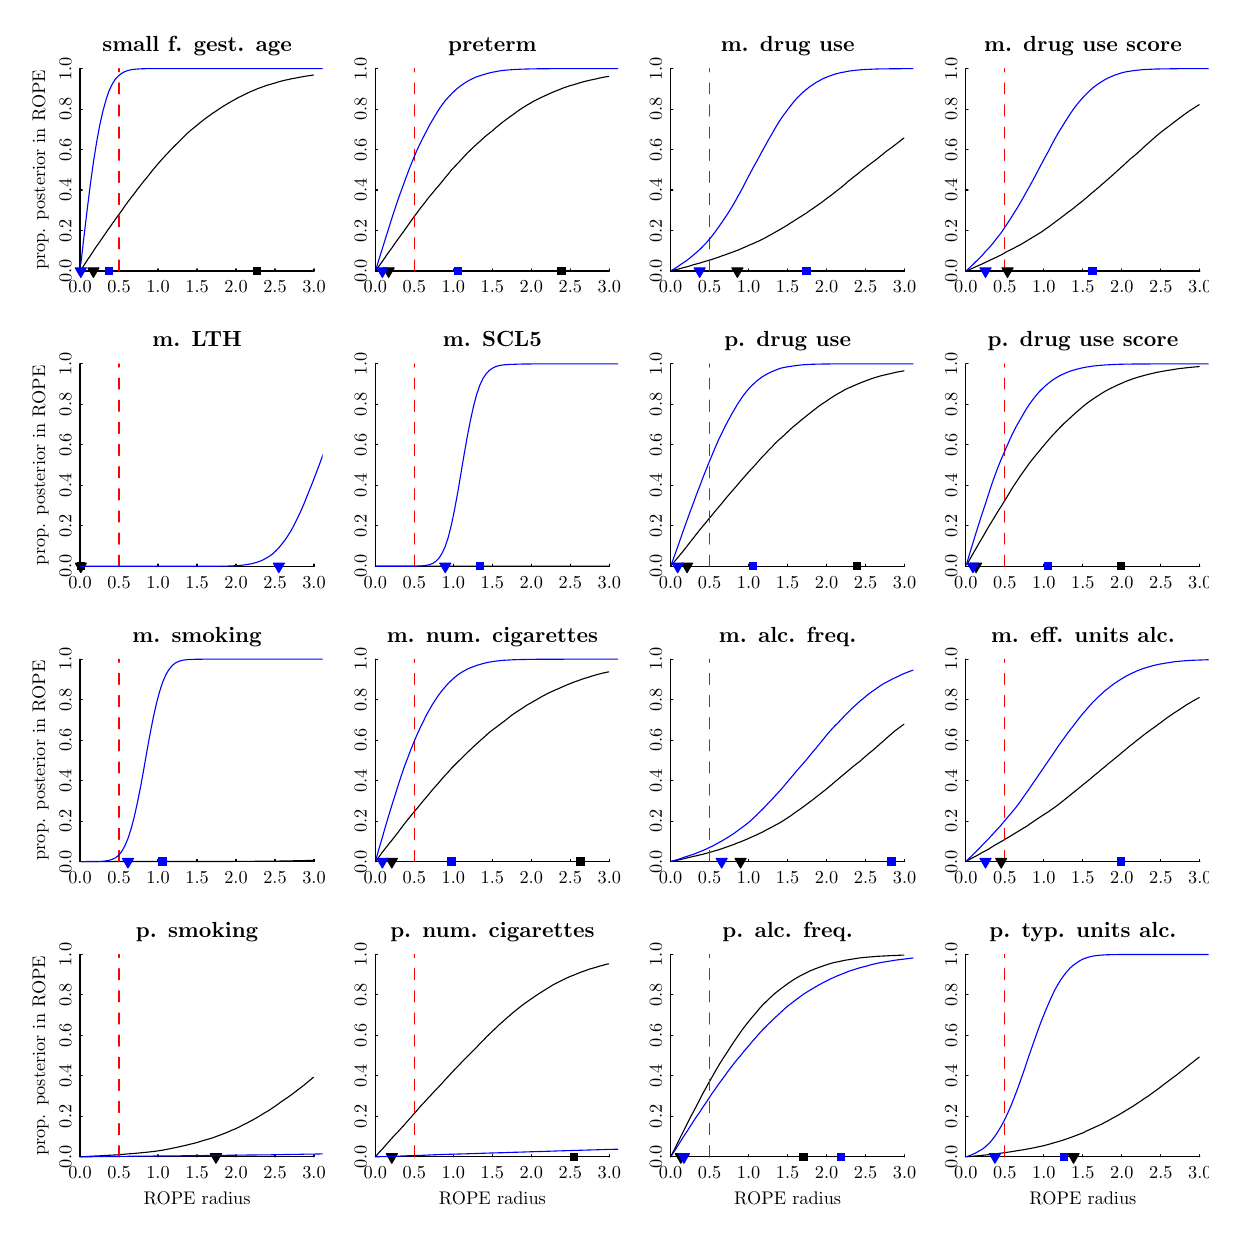
\begin{tikzpicture}[x=1pt,y=1pt]
\definecolor{fillColor}{RGB}{255,255,255}
\path[use as bounding box,fill=fillColor,fill opacity=0.00] (0,0) rectangle (426.79,426.79);
\begin{scope}
\path[clip] ( 15.84,335.93) rectangle (106.62,414.91);
\definecolor{drawColor}{RGB}{0,0,0}

\path[draw=drawColor,line width= 0.4pt,line join=round,line cap=round] ( 19.20,339.21) --
	( 20.34,340.89) --
	( 21.47,342.68) --
	( 22.61,344.35) --
	( 23.75,346.08) --
	( 24.88,347.80) --
	( 26.02,349.38) --
	( 27.15,351.01) --
	( 28.29,352.70) --
	( 29.42,354.34) --
	( 30.56,355.92) --
	( 31.70,357.55) --
	( 32.83,359.13) --
	( 33.97,360.63) --
	( 35.10,362.32) --
	( 36.24,363.87) --
	( 37.38,365.38) --
	( 38.51,366.80) --
	( 39.65,368.37) --
	( 40.78,369.80) --
	( 41.92,371.27) --
	( 43.06,372.59) --
	( 44.19,374.04) --
	( 45.33,375.50) --
	( 46.46,376.84) --
	( 47.60,378.18) --
	( 48.73,379.44) --
	( 49.87,380.68) --
	( 51.01,381.88) --
	( 52.14,383.09) --
	( 53.28,384.26) --
	( 54.41,385.32) --
	( 55.55,386.49) --
	( 56.69,387.62) --
	( 57.82,388.75) --
	( 58.96,389.71) --
	( 60.09,390.65) --
	( 61.23,391.56) --
	( 62.37,392.51) --
	( 63.50,393.40) --
	( 64.64,394.28) --
	( 65.77,395.08) --
	( 66.91,395.91) --
	( 68.04,396.62) --
	( 69.18,397.43) --
	( 70.32,398.15) --
	( 71.45,398.86) --
	( 72.59,399.53) --
	( 73.72,400.19) --
	( 74.86,400.82) --
	( 76.00,401.47) --
	( 77.13,402.02) --
	( 78.27,402.58) --
	( 79.40,403.14) --
	( 80.54,403.68) --
	( 81.67,404.12) --
	( 82.81,404.63) --
	( 83.95,405.06) --
	( 85.08,405.46) --
	( 86.22,405.89) --
	( 87.35,406.22) --
	( 88.49,406.53) --
	( 89.63,406.87) --
	( 90.76,407.23) --
	( 91.90,407.54) --
	( 93.03,407.81) --
	( 94.17,408.04) --
	( 95.31,408.32) --
	( 96.44,408.49) --
	( 97.58,408.74) --
	( 98.71,408.94) --
	( 99.85,409.17) --
	(100.98,409.33) --
	(102.12,409.49) --
	(103.26,409.69);
\end{scope}
\begin{scope}
\path[clip] (  0.00,320.09) rectangle (106.70,426.79);
\definecolor{drawColor}{RGB}{0,0,0}

\node[text=drawColor,rotate= 90.00,anchor=base,inner sep=0pt, outer sep=0pt, scale=  0.66] at (  6.34,375.42) {prop. posterior in ROPE};

\node[text=drawColor,anchor=base,inner sep=0pt, outer sep=0pt, scale=  0.79] at ( 61.23,418.12) {\bfseries small f. gest. age};
\end{scope}
\begin{scope}
\path[clip] (  0.00,  0.00) rectangle (426.79,426.79);
\definecolor{drawColor}{RGB}{0,0,0}

\path[draw=drawColor,line width= 0.4pt,line join=round,line cap=round] ( 18.92,338.86) -- (103.47,338.86);

\path[draw=drawColor,line width= 0.4pt,line join=round,line cap=round] ( 18.92,338.86) -- ( 18.92,339.65);

\path[draw=drawColor,line width= 0.4pt,line join=round,line cap=round] ( 33.01,338.86) -- ( 33.01,339.65);

\path[draw=drawColor,line width= 0.4pt,line join=round,line cap=round] ( 47.10,338.86) -- ( 47.10,339.65);

\path[draw=drawColor,line width= 0.4pt,line join=round,line cap=round] ( 61.20,338.86) -- ( 61.20,339.65);

\path[draw=drawColor,line width= 0.4pt,line join=round,line cap=round] ( 75.29,338.86) -- ( 75.29,339.65);

\path[draw=drawColor,line width= 0.4pt,line join=round,line cap=round] ( 89.38,338.86) -- ( 89.38,339.65);

\path[draw=drawColor,line width= 0.4pt,line join=round,line cap=round] (103.47,338.86) -- (103.47,339.65);

\node[text=drawColor,anchor=base,inner sep=0pt, outer sep=0pt, scale=  0.66] at ( 18.92,330.94) {0.0};

\node[text=drawColor,anchor=base,inner sep=0pt, outer sep=0pt, scale=  0.66] at ( 33.01,330.94) {0.5};

\node[text=drawColor,anchor=base,inner sep=0pt, outer sep=0pt, scale=  0.66] at ( 47.10,330.94) {1.0};

\node[text=drawColor,anchor=base,inner sep=0pt, outer sep=0pt, scale=  0.66] at ( 61.20,330.94) {1.5};

\node[text=drawColor,anchor=base,inner sep=0pt, outer sep=0pt, scale=  0.66] at ( 75.29,330.94) {2.0};

\node[text=drawColor,anchor=base,inner sep=0pt, outer sep=0pt, scale=  0.66] at ( 89.38,330.94) {2.5};

\node[text=drawColor,anchor=base,inner sep=0pt, outer sep=0pt, scale=  0.66] at (103.47,330.94) {3.0};

\path[draw=drawColor,line width= 0.4pt,line join=round,line cap=round] ( 18.92,338.86) -- ( 18.92,411.99);

\path[draw=drawColor,line width= 0.4pt,line join=round,line cap=round] ( 18.92,338.86) -- ( 19.71,338.86);

\path[draw=drawColor,line width= 0.4pt,line join=round,line cap=round] ( 18.92,353.48) -- ( 19.71,353.48);

\path[draw=drawColor,line width= 0.4pt,line join=round,line cap=round] ( 18.92,368.11) -- ( 19.71,368.11);

\path[draw=drawColor,line width= 0.4pt,line join=round,line cap=round] ( 18.92,382.74) -- ( 19.71,382.74);

\path[draw=drawColor,line width= 0.4pt,line join=round,line cap=round] ( 18.92,397.36) -- ( 19.71,397.36);

\path[draw=drawColor,line width= 0.4pt,line join=round,line cap=round] ( 18.92,411.99) -- ( 19.71,411.99);

\node[text=drawColor,rotate= 90.00,anchor=base,inner sep=0pt, outer sep=0pt, scale=  0.66] at ( 15.75,338.86) {0.0};

\node[text=drawColor,rotate= 90.00,anchor=base,inner sep=0pt, outer sep=0pt, scale=  0.66] at ( 15.75,353.48) {0.2};

\node[text=drawColor,rotate= 90.00,anchor=base,inner sep=0pt, outer sep=0pt, scale=  0.66] at ( 15.75,368.11) {0.4};

\node[text=drawColor,rotate= 90.00,anchor=base,inner sep=0pt, outer sep=0pt, scale=  0.66] at ( 15.75,382.74) {0.6};

\node[text=drawColor,rotate= 90.00,anchor=base,inner sep=0pt, outer sep=0pt, scale=  0.66] at ( 15.75,397.36) {0.8};

\node[text=drawColor,rotate= 90.00,anchor=base,inner sep=0pt, outer sep=0pt, scale=  0.66] at ( 15.75,411.99) {1.0};
\end{scope}
\begin{scope}
\path[clip] ( 15.84,335.93) rectangle (106.62,414.91);
\definecolor{drawColor}{RGB}{0,0,0}

\path[draw=drawColor,line width= 0.4pt,line join=round,line cap=round] (131.65,338.86) --
	(131.65,411.99);
\definecolor{drawColor}{RGB}{255,0,0}

\path[draw=drawColor,line width= 0.4pt,dash pattern=on 4pt off 4pt ,line join=round,line cap=round] ( 33.01,338.86) --
	( 33.01,411.99);
\definecolor{fillColor}{RGB}{0,0,0}

\path[fill=fillColor] ( 81.33,337.37) --
	( 84.30,337.37) --
	( 84.30,340.34) --
	( 81.33,340.34) --
	cycle;
\definecolor{drawColor}{RGB}{0,0,0}

\path[draw=drawColor,line width= 0.4pt,line join=round,line cap=round,fill=fillColor] ( 23.75,336.55) --
	( 25.75,340.01) --
	( 21.75,340.01) --
	cycle;
\definecolor{drawColor}{RGB}{0,0,255}

\path[draw=drawColor,line width= 0.4pt,line join=round,line cap=round] ( 19.20,341.27) --
	( 20.34,351.26) --
	( 21.47,360.79) --
	( 22.61,369.87) --
	( 23.75,378.15) --
	( 24.88,385.22) --
	( 26.02,391.44) --
	( 27.15,396.48) --
	( 28.29,400.64) --
	( 29.42,404.01) --
	( 30.56,406.41) --
	( 31.70,408.19) --
	( 32.83,409.41) --
	( 33.97,410.28) --
	( 35.10,410.89) --
	( 36.24,411.32) --
	( 37.38,411.60) --
	( 38.51,411.74) --
	( 39.65,411.84) --
	( 40.78,411.91) --
	( 41.92,411.95) --
	( 43.06,411.98) --
	( 44.19,411.98) --
	( 45.33,411.98) --
	( 46.46,411.98) --
	( 47.60,411.98) --
	( 48.73,411.98) --
	( 49.87,411.99) --
	( 51.01,411.99) --
	( 52.14,411.99) --
	( 53.28,411.99) --
	( 54.41,411.99) --
	( 55.55,411.99) --
	( 56.69,411.99) --
	( 57.82,411.99) --
	( 58.96,411.99) --
	( 60.09,411.99) --
	( 61.23,411.99) --
	( 62.37,411.99) --
	( 63.50,411.99) --
	( 64.64,411.99) --
	( 65.77,411.99) --
	( 66.91,411.99) --
	( 68.04,411.99) --
	( 69.18,411.99) --
	( 70.32,411.99) --
	( 71.45,411.99) --
	( 72.59,411.99) --
	( 73.72,411.99) --
	( 74.86,411.99) --
	( 76.00,411.99) --
	( 77.13,411.99) --
	( 78.27,411.99) --
	( 79.40,411.99) --
	( 80.54,411.99) --
	( 81.67,411.99) --
	( 82.81,411.99) --
	( 83.95,411.99) --
	( 85.08,411.99) --
	( 86.22,411.99) --
	( 87.35,411.99) --
	( 88.49,411.99) --
	( 89.63,411.99) --
	( 90.76,411.99) --
	( 91.90,411.99) --
	( 93.03,411.99) --
	( 94.17,411.99) --
	( 95.31,411.99) --
	( 96.44,411.99) --
	( 97.58,411.99) --
	( 98.71,411.99) --
	( 99.85,411.99) --
	(100.98,411.99) --
	(102.12,411.99) --
	(103.26,411.99) --
	(104.39,411.99) --
	(105.53,411.99) --
	(106.66,411.99) --
	(107.80,411.99) --
	(108.94,411.99) --
	(110.07,411.99) --
	(111.21,411.99) --
	(112.34,411.99) --
	(113.48,411.99) --
	(114.62,411.99) --
	(115.75,411.99) --
	(116.89,411.99) --
	(118.02,411.99) --
	(119.16,411.99) --
	(120.29,411.99) --
	(121.43,411.99) --
	(122.57,411.99) --
	(123.70,411.99) --
	(124.84,411.99) --
	(125.97,411.99) --
	(127.11,411.99) --
	(128.25,411.99) --
	(129.38,411.99) --
	(130.52,411.99) --
	(131.65,411.99);
\definecolor{fillColor}{RGB}{0,0,255}

\path[fill=fillColor] ( 27.94,337.37) --
	( 30.91,337.37) --
	( 30.91,340.34) --
	( 27.94,340.34) --
	cycle;

\path[draw=drawColor,line width= 0.4pt,line join=round,line cap=round,fill=fillColor] ( 19.20,336.55) --
	( 21.20,340.01) --
	( 17.20,340.01) --
	cycle;
\end{scope}
\begin{scope}
\path[clip] (122.54,335.93) rectangle (213.32,414.91);
\definecolor{drawColor}{RGB}{0,0,0}

\path[draw=drawColor,line width= 0.4pt,line join=round,line cap=round] (125.90,339.19) --
	(127.04,340.76) --
	(128.17,342.37) --
	(129.31,344.00) --
	(130.44,345.65) --
	(131.58,347.16) --
	(132.72,348.86) --
	(133.85,350.41) --
	(134.99,351.98) --
	(136.12,353.50) --
	(137.26,355.16) --
	(138.39,356.73) --
	(139.53,358.36) --
	(140.67,359.85) --
	(141.80,361.42) --
	(142.94,362.84) --
	(144.07,364.32) --
	(145.21,365.77) --
	(146.35,367.12) --
	(147.48,368.52) --
	(148.62,369.79) --
	(149.75,371.19) --
	(150.89,372.62) --
	(152.02,373.93) --
	(153.16,375.39) --
	(154.30,376.59) --
	(155.43,377.76) --
	(156.57,378.99) --
	(157.70,380.24) --
	(158.84,381.44) --
	(159.98,382.55) --
	(161.11,383.64) --
	(162.25,384.68) --
	(163.38,385.68) --
	(164.52,386.72) --
	(165.66,387.75) --
	(166.79,388.63) --
	(167.93,389.52) --
	(169.06,390.55) --
	(170.20,391.46) --
	(171.33,392.41) --
	(172.47,393.27) --
	(173.61,394.11) --
	(174.74,394.94) --
	(175.88,395.73) --
	(177.01,396.58) --
	(178.15,397.37) --
	(179.29,398.11) --
	(180.42,398.80) --
	(181.56,399.44) --
	(182.69,400.12) --
	(183.83,400.68) --
	(184.97,401.28) --
	(186.10,401.81) --
	(187.24,402.33) --
	(188.37,402.86) --
	(189.51,403.34) --
	(190.64,403.84) --
	(191.78,404.27) --
	(192.92,404.73) --
	(194.05,405.18) --
	(195.19,405.57) --
	(196.32,405.91) --
	(197.46,406.22) --
	(198.60,406.58) --
	(199.73,406.93) --
	(200.87,407.25) --
	(202.00,407.53) --
	(203.14,407.80) --
	(204.27,408.04) --
	(205.41,408.28) --
	(206.55,408.56) --
	(207.68,408.80) --
	(208.82,409.01) --
	(209.95,409.16);
\end{scope}
\begin{scope}
\path[clip] (106.70,320.09) rectangle (213.40,426.79);
\definecolor{drawColor}{RGB}{0,0,0}

\node[text=drawColor,anchor=base,inner sep=0pt, outer sep=0pt, scale=  0.79] at (167.93,418.12) {\bfseries preterm};
\end{scope}
\begin{scope}
\path[clip] (  0.00,  0.00) rectangle (426.79,426.79);
\definecolor{drawColor}{RGB}{0,0,0}

\path[draw=drawColor,line width= 0.4pt,line join=round,line cap=round] (125.62,338.86) -- (210.17,338.86);

\path[draw=drawColor,line width= 0.4pt,line join=round,line cap=round] (125.62,338.86) -- (125.62,339.65);

\path[draw=drawColor,line width= 0.4pt,line join=round,line cap=round] (139.71,338.86) -- (139.71,339.65);

\path[draw=drawColor,line width= 0.4pt,line join=round,line cap=round] (153.80,338.86) -- (153.80,339.65);

\path[draw=drawColor,line width= 0.4pt,line join=round,line cap=round] (167.89,338.86) -- (167.89,339.65);

\path[draw=drawColor,line width= 0.4pt,line join=round,line cap=round] (181.98,338.86) -- (181.98,339.65);

\path[draw=drawColor,line width= 0.4pt,line join=round,line cap=round] (196.08,338.86) -- (196.08,339.65);

\path[draw=drawColor,line width= 0.4pt,line join=round,line cap=round] (210.17,338.86) -- (210.17,339.65);

\node[text=drawColor,anchor=base,inner sep=0pt, outer sep=0pt, scale=  0.66] at (125.62,330.94) {0.0};

\node[text=drawColor,anchor=base,inner sep=0pt, outer sep=0pt, scale=  0.66] at (139.71,330.94) {0.5};

\node[text=drawColor,anchor=base,inner sep=0pt, outer sep=0pt, scale=  0.66] at (153.80,330.94) {1.0};

\node[text=drawColor,anchor=base,inner sep=0pt, outer sep=0pt, scale=  0.66] at (167.89,330.94) {1.5};

\node[text=drawColor,anchor=base,inner sep=0pt, outer sep=0pt, scale=  0.66] at (181.98,330.94) {2.0};

\node[text=drawColor,anchor=base,inner sep=0pt, outer sep=0pt, scale=  0.66] at (196.08,330.94) {2.5};

\node[text=drawColor,anchor=base,inner sep=0pt, outer sep=0pt, scale=  0.66] at (210.17,330.94) {3.0};

\path[draw=drawColor,line width= 0.4pt,line join=round,line cap=round] (125.62,338.86) -- (125.62,411.99);

\path[draw=drawColor,line width= 0.4pt,line join=round,line cap=round] (125.62,338.86) -- (126.41,338.86);

\path[draw=drawColor,line width= 0.4pt,line join=round,line cap=round] (125.62,353.48) -- (126.41,353.48);

\path[draw=drawColor,line width= 0.4pt,line join=round,line cap=round] (125.62,368.11) -- (126.41,368.11);

\path[draw=drawColor,line width= 0.4pt,line join=round,line cap=round] (125.62,382.74) -- (126.41,382.74);

\path[draw=drawColor,line width= 0.4pt,line join=round,line cap=round] (125.62,397.36) -- (126.41,397.36);

\path[draw=drawColor,line width= 0.4pt,line join=round,line cap=round] (125.62,411.99) -- (126.41,411.99);

\node[text=drawColor,rotate= 90.00,anchor=base,inner sep=0pt, outer sep=0pt, scale=  0.66] at (122.45,338.86) {0.0};

\node[text=drawColor,rotate= 90.00,anchor=base,inner sep=0pt, outer sep=0pt, scale=  0.66] at (122.45,353.48) {0.2};

\node[text=drawColor,rotate= 90.00,anchor=base,inner sep=0pt, outer sep=0pt, scale=  0.66] at (122.45,368.11) {0.4};

\node[text=drawColor,rotate= 90.00,anchor=base,inner sep=0pt, outer sep=0pt, scale=  0.66] at (122.45,382.74) {0.6};

\node[text=drawColor,rotate= 90.00,anchor=base,inner sep=0pt, outer sep=0pt, scale=  0.66] at (122.45,397.36) {0.8};

\node[text=drawColor,rotate= 90.00,anchor=base,inner sep=0pt, outer sep=0pt, scale=  0.66] at (122.45,411.99) {1.0};
\end{scope}
\begin{scope}
\path[clip] (122.54,335.93) rectangle (213.32,414.91);
\definecolor{drawColor}{RGB}{0,0,0}

\path[draw=drawColor,line width= 0.4pt,line join=round,line cap=round] (238.35,338.86) --
	(238.35,411.99);
\definecolor{drawColor}{RGB}{255,0,0}

\path[draw=drawColor,line width= 0.4pt,dash pattern=on 4pt off 4pt ,line join=round,line cap=round] (139.71,338.86) --
	(139.71,411.99);
\definecolor{fillColor}{RGB}{0,0,0}

\path[fill=fillColor] (191.43,337.37) --
	(194.40,337.37) --
	(194.40,340.34) --
	(191.43,340.34) --
	cycle;
\definecolor{drawColor}{RGB}{0,0,0}

\path[draw=drawColor,line width= 0.4pt,line join=round,line cap=round,fill=fillColor] (130.44,336.55) --
	(132.44,340.01) --
	(128.44,340.01) --
	cycle;
\definecolor{drawColor}{RGB}{0,0,255}

\path[draw=drawColor,line width= 0.4pt,line join=round,line cap=round] (125.90,339.68) --
	(127.04,343.34) --
	(128.17,347.00) --
	(129.31,350.66) --
	(130.44,354.20) --
	(131.58,357.88) --
	(132.72,361.39) --
	(133.85,364.72) --
	(134.99,367.88) --
	(136.12,370.99) --
	(137.26,374.07) --
	(138.39,377.01) --
	(139.53,379.81) --
	(140.67,382.49) --
	(141.80,384.88) --
	(142.94,387.21) --
	(144.07,389.32) --
	(145.21,391.53) --
	(146.35,393.53) --
	(147.48,395.42) --
	(148.62,397.27) --
	(149.75,398.92) --
	(150.89,400.39) --
	(152.02,401.65) --
	(153.16,402.86) --
	(154.30,403.97) --
	(155.43,404.98) --
	(156.57,405.87) --
	(157.70,406.63) --
	(158.84,407.36) --
	(159.98,407.97) --
	(161.11,408.54) --
	(162.25,409.03) --
	(163.38,409.41) --
	(164.52,409.77) --
	(165.66,410.11) --
	(166.79,410.41) --
	(167.93,410.68) --
	(169.06,410.88) --
	(170.20,411.11) --
	(171.33,411.27) --
	(172.47,411.41) --
	(173.61,411.51) --
	(174.74,411.59) --
	(175.88,411.65) --
	(177.01,411.71) --
	(178.15,411.78) --
	(179.29,411.82) --
	(180.42,411.85) --
	(181.56,411.88) --
	(182.69,411.90) --
	(183.83,411.92) --
	(184.97,411.94) --
	(186.10,411.95) --
	(187.24,411.95) --
	(188.37,411.96) --
	(189.51,411.97) --
	(190.64,411.97) --
	(191.78,411.97) --
	(192.92,411.98) --
	(194.05,411.98) --
	(195.19,411.98) --
	(196.32,411.98) --
	(197.46,411.98) --
	(198.60,411.98) --
	(199.73,411.98) --
	(200.87,411.98) --
	(202.00,411.98) --
	(203.14,411.98) --
	(204.27,411.98) --
	(205.41,411.99) --
	(206.55,411.99) --
	(207.68,411.99) --
	(208.82,411.99) --
	(209.95,411.99) --
	(211.09,411.99) --
	(212.23,411.99) --
	(213.36,411.99) --
	(214.50,411.99) --
	(215.63,411.99) --
	(216.77,411.99) --
	(217.91,411.99) --
	(219.04,411.99) --
	(220.18,411.99) --
	(221.31,411.99) --
	(222.45,411.99) --
	(223.58,411.99) --
	(224.72,411.99) --
	(225.86,411.99) --
	(226.99,411.99) --
	(228.13,411.99) --
	(229.26,411.99) --
	(230.40,411.99) --
	(231.54,411.99) --
	(232.67,411.99) --
	(233.81,411.99) --
	(234.94,411.99) --
	(236.08,411.99) --
	(237.22,411.99) --
	(238.35,411.99);
\definecolor{fillColor}{RGB}{0,0,255}

\path[fill=fillColor] (153.95,337.37) --
	(156.92,337.37) --
	(156.92,340.34) --
	(153.95,340.34) --
	cycle;

\path[draw=drawColor,line width= 0.4pt,line join=round,line cap=round,fill=fillColor] (128.17,336.55) --
	(130.17,340.01) --
	(126.17,340.01) --
	cycle;
\end{scope}
\begin{scope}
\path[clip] (229.24,335.93) rectangle (320.01,414.91);
\definecolor{drawColor}{RGB}{0,0,0}

\path[draw=drawColor,line width= 0.4pt,line join=round,line cap=round] (232.60,338.94) --
	(233.73,339.24) --
	(234.87,339.50) --
	(236.01,339.80) --
	(237.14,340.12) --
	(238.28,340.40) --
	(239.41,340.74) --
	(240.55,341.12) --
	(241.68,341.41) --
	(242.82,341.72) --
	(243.96,342.07) --
	(245.09,342.41) --
	(246.23,342.74) --
	(247.36,343.08) --
	(248.50,343.48) --
	(249.64,343.85) --
	(250.77,344.28) --
	(251.91,344.66) --
	(253.04,345.08) --
	(254.18,345.49) --
	(255.32,345.92) --
	(256.45,346.33) --
	(257.59,346.81) --
	(258.72,347.31) --
	(259.86,347.79) --
	(260.99,348.33) --
	(262.13,348.76) --
	(263.27,349.30) --
	(264.40,349.78) --
	(265.54,350.37) --
	(266.67,350.95) --
	(267.81,351.59) --
	(268.95,352.20) --
	(270.08,352.86) --
	(271.22,353.52) --
	(272.35,354.15) --
	(273.49,354.82) --
	(274.62,355.50) --
	(275.76,356.26) --
	(276.90,356.96) --
	(278.03,357.70) --
	(279.17,358.40) --
	(280.30,359.11) --
	(281.44,359.84) --
	(282.58,360.68) --
	(283.71,361.42) --
	(284.85,362.24) --
	(285.98,363.01) --
	(287.12,363.81) --
	(288.26,364.71) --
	(289.39,365.56) --
	(290.53,366.37) --
	(291.66,367.29) --
	(292.80,368.16) --
	(293.93,369.03) --
	(295.07,369.99) --
	(296.21,371.02) --
	(297.34,371.91) --
	(298.48,372.85) --
	(299.61,373.69) --
	(300.75,374.65) --
	(301.89,375.56) --
	(303.02,376.44) --
	(304.16,377.30) --
	(305.29,378.16) --
	(306.43,378.98) --
	(307.57,379.91) --
	(308.70,380.81) --
	(309.84,381.77) --
	(310.97,382.61) --
	(312.11,383.43) --
	(313.24,384.28) --
	(314.38,385.18) --
	(315.52,386.05) --
	(316.65,386.94);
\end{scope}
\begin{scope}
\path[clip] (213.40,320.09) rectangle (320.09,426.79);
\definecolor{drawColor}{RGB}{0,0,0}

\node[text=drawColor,anchor=base,inner sep=0pt, outer sep=0pt, scale=  0.79] at (274.62,418.12) {\bfseries m. drug use};
\end{scope}
\begin{scope}
\path[clip] (  0.00,  0.00) rectangle (426.79,426.79);
\definecolor{drawColor}{RGB}{0,0,0}

\path[draw=drawColor,line width= 0.4pt,line join=round,line cap=round] (232.32,338.86) -- (316.87,338.86);

\path[draw=drawColor,line width= 0.4pt,line join=round,line cap=round] (232.32,338.86) -- (232.32,339.65);

\path[draw=drawColor,line width= 0.4pt,line join=round,line cap=round] (246.41,338.86) -- (246.41,339.65);

\path[draw=drawColor,line width= 0.4pt,line join=round,line cap=round] (260.50,338.86) -- (260.50,339.65);

\path[draw=drawColor,line width= 0.4pt,line join=round,line cap=round] (274.59,338.86) -- (274.59,339.65);

\path[draw=drawColor,line width= 0.4pt,line join=round,line cap=round] (288.68,338.86) -- (288.68,339.65);

\path[draw=drawColor,line width= 0.4pt,line join=round,line cap=round] (302.77,338.86) -- (302.77,339.65);

\path[draw=drawColor,line width= 0.4pt,line join=round,line cap=round] (316.87,338.86) -- (316.87,339.65);

\node[text=drawColor,anchor=base,inner sep=0pt, outer sep=0pt, scale=  0.66] at (232.32,330.94) {0.0};

\node[text=drawColor,anchor=base,inner sep=0pt, outer sep=0pt, scale=  0.66] at (246.41,330.94) {0.5};

\node[text=drawColor,anchor=base,inner sep=0pt, outer sep=0pt, scale=  0.66] at (260.50,330.94) {1.0};

\node[text=drawColor,anchor=base,inner sep=0pt, outer sep=0pt, scale=  0.66] at (274.59,330.94) {1.5};

\node[text=drawColor,anchor=base,inner sep=0pt, outer sep=0pt, scale=  0.66] at (288.68,330.94) {2.0};

\node[text=drawColor,anchor=base,inner sep=0pt, outer sep=0pt, scale=  0.66] at (302.77,330.94) {2.5};

\node[text=drawColor,anchor=base,inner sep=0pt, outer sep=0pt, scale=  0.66] at (316.87,330.94) {3.0};

\path[draw=drawColor,line width= 0.4pt,line join=round,line cap=round] (232.32,338.86) -- (232.32,411.99);

\path[draw=drawColor,line width= 0.4pt,line join=round,line cap=round] (232.32,338.86) -- (233.11,338.86);

\path[draw=drawColor,line width= 0.4pt,line join=round,line cap=round] (232.32,353.48) -- (233.11,353.48);

\path[draw=drawColor,line width= 0.4pt,line join=round,line cap=round] (232.32,368.11) -- (233.11,368.11);

\path[draw=drawColor,line width= 0.4pt,line join=round,line cap=round] (232.32,382.74) -- (233.11,382.74);

\path[draw=drawColor,line width= 0.4pt,line join=round,line cap=round] (232.32,397.36) -- (233.11,397.36);

\path[draw=drawColor,line width= 0.4pt,line join=round,line cap=round] (232.32,411.99) -- (233.11,411.99);

\node[text=drawColor,rotate= 90.00,anchor=base,inner sep=0pt, outer sep=0pt, scale=  0.66] at (229.15,338.86) {0.0};

\node[text=drawColor,rotate= 90.00,anchor=base,inner sep=0pt, outer sep=0pt, scale=  0.66] at (229.15,353.48) {0.2};

\node[text=drawColor,rotate= 90.00,anchor=base,inner sep=0pt, outer sep=0pt, scale=  0.66] at (229.15,368.11) {0.4};

\node[text=drawColor,rotate= 90.00,anchor=base,inner sep=0pt, outer sep=0pt, scale=  0.66] at (229.15,382.74) {0.6};

\node[text=drawColor,rotate= 90.00,anchor=base,inner sep=0pt, outer sep=0pt, scale=  0.66] at (229.15,397.36) {0.8};

\node[text=drawColor,rotate= 90.00,anchor=base,inner sep=0pt, outer sep=0pt, scale=  0.66] at (229.15,411.99) {1.0};
\end{scope}
\begin{scope}
\path[clip] (229.24,335.93) rectangle (320.01,414.91);
\definecolor{drawColor}{RGB}{0,0,0}

\path[draw=drawColor,line width= 0.4pt,line join=round,line cap=round] (345.05,338.86) --
	(345.05,411.99);
\definecolor{drawColor}{RGB}{255,0,0}

\path[draw=drawColor,line width= 0.4pt,dash pattern=on 4pt off 4pt ,line join=round,line cap=round] (246.41,338.86) --
	(246.41,411.99);
\definecolor{fillColor}{RGB}{0,0,0}

\path[fill=fillColor] (343.56,337.37) --
	(346.53,337.37) --
	(346.53,340.34) --
	(343.56,340.34) --
	cycle;
\definecolor{drawColor}{RGB}{0,0,0}

\path[draw=drawColor,line width= 0.4pt,line join=round,line cap=round,fill=fillColor] (256.45,336.55) --
	(258.45,340.01) --
	(254.45,340.01) --
	cycle;
\definecolor{drawColor}{RGB}{0,0,255}

\path[draw=drawColor,line width= 0.4pt,line join=round,line cap=round] (232.60,339.05) --
	(233.73,339.69) --
	(234.87,340.42) --
	(236.01,341.25) --
	(237.14,341.99) --
	(238.28,342.77) --
	(239.41,343.67) --
	(240.55,344.61) --
	(241.68,345.58) --
	(242.82,346.60) --
	(243.96,347.75) --
	(245.09,348.91) --
	(246.23,350.20) --
	(247.36,351.59) --
	(248.50,353.11) --
	(249.64,354.68) --
	(250.77,356.33) --
	(251.91,358.01) --
	(253.04,359.69) --
	(254.18,361.54) --
	(255.32,363.41) --
	(256.45,365.49) --
	(257.59,367.49) --
	(258.72,369.61) --
	(259.86,371.89) --
	(260.99,374.02) --
	(262.13,376.19) --
	(263.27,378.19) --
	(264.40,380.26) --
	(265.54,382.41) --
	(266.67,384.41) --
	(267.81,386.51) --
	(268.95,388.41) --
	(270.08,390.42) --
	(271.22,392.34) --
	(272.35,394.08) --
	(273.49,395.65) --
	(274.62,397.19) --
	(275.76,398.64) --
	(276.90,400.10) --
	(278.03,401.41) --
	(279.17,402.51) --
	(280.30,403.59) --
	(281.44,404.51) --
	(282.58,405.43) --
	(283.71,406.18) --
	(284.85,406.96) --
	(285.98,407.58) --
	(287.12,408.23) --
	(288.26,408.73) --
	(289.39,409.20) --
	(290.53,409.59) --
	(291.66,409.98) --
	(292.80,410.28) --
	(293.93,410.56) --
	(295.07,410.75) --
	(296.21,410.99) --
	(297.34,411.17) --
	(298.48,411.30) --
	(299.61,411.44) --
	(300.75,411.55) --
	(301.89,411.63) --
	(303.02,411.69) --
	(304.16,411.74) --
	(305.29,411.79) --
	(306.43,411.84) --
	(307.57,411.87) --
	(308.70,411.89) --
	(309.84,411.91) --
	(310.97,411.92) --
	(312.11,411.93) --
	(313.24,411.94) --
	(314.38,411.95) --
	(315.52,411.96) --
	(316.65,411.97) --
	(317.79,411.97) --
	(318.92,411.98) --
	(320.06,411.98) --
	(321.20,411.98) --
	(322.33,411.98) --
	(323.47,411.99) --
	(324.60,411.99) --
	(325.74,411.99) --
	(326.87,411.99) --
	(328.01,411.99) --
	(329.15,411.99) --
	(330.28,411.99) --
	(331.42,411.99) --
	(332.55,411.99) --
	(333.69,411.99) --
	(334.83,411.99) --
	(335.96,411.99) --
	(337.10,411.99) --
	(338.23,411.99) --
	(339.37,411.99) --
	(340.51,411.99) --
	(341.64,411.99) --
	(342.78,411.99) --
	(343.91,411.99) --
	(345.05,411.99);
\definecolor{fillColor}{RGB}{0,0,255}

\path[fill=fillColor] (279.96,337.37) --
	(282.93,337.37) --
	(282.93,340.34) --
	(279.96,340.34) --
	cycle;

\path[draw=drawColor,line width= 0.4pt,line join=round,line cap=round,fill=fillColor] (242.82,336.55) --
	(244.82,340.01) --
	(240.82,340.01) --
	cycle;
\end{scope}
\begin{scope}
\path[clip] (335.93,335.93) rectangle (426.71,414.91);
\definecolor{drawColor}{RGB}{0,0,0}

\path[draw=drawColor,line width= 0.4pt,line join=round,line cap=round] (339.30,339.00) --
	(340.43,339.43) --
	(341.57,339.93) --
	(342.70,340.43) --
	(343.84,340.96) --
	(344.98,341.44) --
	(346.11,342.01) --
	(347.25,342.53) --
	(348.38,343.07) --
	(349.52,343.60) --
	(350.65,344.12) --
	(351.79,344.68) --
	(352.93,345.35) --
	(354.06,346.00) --
	(355.20,346.55) --
	(356.33,347.09) --
	(357.47,347.73) --
	(358.61,348.30) --
	(359.74,348.95) --
	(360.88,349.65) --
	(362.01,350.34) --
	(363.15,351.04) --
	(364.28,351.71) --
	(365.42,352.41) --
	(366.56,353.12) --
	(367.69,353.95) --
	(368.83,354.71) --
	(369.96,355.57) --
	(371.10,356.42) --
	(372.24,357.27) --
	(373.37,358.12) --
	(374.51,358.97) --
	(375.64,359.89) --
	(376.78,360.69) --
	(377.92,361.54) --
	(379.05,362.50) --
	(380.19,363.38) --
	(381.32,364.28) --
	(382.46,365.23) --
	(383.59,366.21) --
	(384.73,367.21) --
	(385.87,368.13) --
	(387.00,369.09) --
	(388.14,370.13) --
	(389.27,371.07) --
	(390.41,372.09) --
	(391.55,373.05) --
	(392.68,374.08) --
	(393.82,375.11) --
	(394.95,376.17) --
	(396.09,377.13) --
	(397.22,378.23) --
	(398.36,379.30) --
	(399.50,380.20) --
	(400.63,381.15) --
	(401.77,382.16) --
	(402.90,383.22) --
	(404.04,384.30) --
	(405.18,385.28) --
	(406.31,386.27) --
	(407.45,387.28) --
	(408.58,388.25) --
	(409.72,389.18) --
	(410.86,390.05) --
	(411.99,390.89) --
	(413.13,391.76) --
	(414.26,392.64) --
	(415.40,393.51) --
	(416.53,394.34) --
	(417.67,395.21) --
	(418.81,396.01) --
	(419.94,396.83) --
	(421.08,397.53) --
	(422.21,398.28) --
	(423.35,398.98);
\end{scope}
\begin{scope}
\path[clip] (320.09,320.09) rectangle (426.79,426.79);
\definecolor{drawColor}{RGB}{0,0,0}

\node[text=drawColor,anchor=base,inner sep=0pt, outer sep=0pt, scale=  0.79] at (381.32,418.12) {\bfseries m. drug use score};
\end{scope}
\begin{scope}
\path[clip] (  0.00,  0.00) rectangle (426.79,426.79);
\definecolor{drawColor}{RGB}{0,0,0}

\path[draw=drawColor,line width= 0.4pt,line join=round,line cap=round] (339.01,338.86) -- (423.56,338.86);

\path[draw=drawColor,line width= 0.4pt,line join=round,line cap=round] (339.01,338.86) -- (339.01,339.65);

\path[draw=drawColor,line width= 0.4pt,line join=round,line cap=round] (353.11,338.86) -- (353.11,339.65);

\path[draw=drawColor,line width= 0.4pt,line join=round,line cap=round] (367.20,338.86) -- (367.20,339.65);

\path[draw=drawColor,line width= 0.4pt,line join=round,line cap=round] (381.29,338.86) -- (381.29,339.65);

\path[draw=drawColor,line width= 0.4pt,line join=round,line cap=round] (395.38,338.86) -- (395.38,339.65);

\path[draw=drawColor,line width= 0.4pt,line join=round,line cap=round] (409.47,338.86) -- (409.47,339.65);

\path[draw=drawColor,line width= 0.4pt,line join=round,line cap=round] (423.56,338.86) -- (423.56,339.65);

\node[text=drawColor,anchor=base,inner sep=0pt, outer sep=0pt, scale=  0.66] at (339.01,330.94) {0.0};

\node[text=drawColor,anchor=base,inner sep=0pt, outer sep=0pt, scale=  0.66] at (353.11,330.94) {0.5};

\node[text=drawColor,anchor=base,inner sep=0pt, outer sep=0pt, scale=  0.66] at (367.20,330.94) {1.0};

\node[text=drawColor,anchor=base,inner sep=0pt, outer sep=0pt, scale=  0.66] at (381.29,330.94) {1.5};

\node[text=drawColor,anchor=base,inner sep=0pt, outer sep=0pt, scale=  0.66] at (395.38,330.94) {2.0};

\node[text=drawColor,anchor=base,inner sep=0pt, outer sep=0pt, scale=  0.66] at (409.47,330.94) {2.5};

\node[text=drawColor,anchor=base,inner sep=0pt, outer sep=0pt, scale=  0.66] at (423.56,330.94) {3.0};

\path[draw=drawColor,line width= 0.4pt,line join=round,line cap=round] (339.01,338.86) -- (339.01,411.99);

\path[draw=drawColor,line width= 0.4pt,line join=round,line cap=round] (339.01,338.86) -- (339.80,338.86);

\path[draw=drawColor,line width= 0.4pt,line join=round,line cap=round] (339.01,353.48) -- (339.80,353.48);

\path[draw=drawColor,line width= 0.4pt,line join=round,line cap=round] (339.01,368.11) -- (339.80,368.11);

\path[draw=drawColor,line width= 0.4pt,line join=round,line cap=round] (339.01,382.74) -- (339.80,382.74);

\path[draw=drawColor,line width= 0.4pt,line join=round,line cap=round] (339.01,397.36) -- (339.80,397.36);

\path[draw=drawColor,line width= 0.4pt,line join=round,line cap=round] (339.01,411.99) -- (339.80,411.99);

\node[text=drawColor,rotate= 90.00,anchor=base,inner sep=0pt, outer sep=0pt, scale=  0.66] at (335.85,338.86) {0.0};

\node[text=drawColor,rotate= 90.00,anchor=base,inner sep=0pt, outer sep=0pt, scale=  0.66] at (335.85,353.48) {0.2};

\node[text=drawColor,rotate= 90.00,anchor=base,inner sep=0pt, outer sep=0pt, scale=  0.66] at (335.85,368.11) {0.4};

\node[text=drawColor,rotate= 90.00,anchor=base,inner sep=0pt, outer sep=0pt, scale=  0.66] at (335.85,382.74) {0.6};

\node[text=drawColor,rotate= 90.00,anchor=base,inner sep=0pt, outer sep=0pt, scale=  0.66] at (335.85,397.36) {0.8};

\node[text=drawColor,rotate= 90.00,anchor=base,inner sep=0pt, outer sep=0pt, scale=  0.66] at (335.85,411.99) {1.0};
\end{scope}
\begin{scope}
\path[clip] (335.93,335.93) rectangle (426.71,414.91);
\definecolor{drawColor}{RGB}{255,0,0}

\path[draw=drawColor,line width= 0.4pt,dash pattern=on 4pt off 4pt ,line join=round,line cap=round] (353.11,338.86) --
	(353.11,411.99);
\definecolor{drawColor}{RGB}{0,0,0}
\definecolor{fillColor}{RGB}{0,0,0}

\path[draw=drawColor,line width= 0.4pt,line join=round,line cap=round,fill=fillColor] (354.06,336.55) --
	(356.06,340.01) --
	(352.06,340.01) --
	cycle;
\definecolor{drawColor}{RGB}{0,0,255}

\path[draw=drawColor,line width= 0.4pt,line join=round,line cap=round] (339.30,339.10) --
	(340.43,340.12) --
	(341.57,341.20) --
	(342.70,342.31) --
	(343.84,343.44) --
	(344.98,344.57) --
	(346.11,345.93) --
	(347.25,347.09) --
	(348.38,348.36) --
	(349.52,349.81) --
	(350.65,351.28) --
	(351.79,352.71) --
	(352.93,354.38) --
	(354.06,356.09) --
	(355.20,357.84) --
	(356.33,359.68) --
	(357.47,361.47) --
	(358.61,363.41) --
	(359.74,365.36) --
	(360.88,367.45) --
	(362.01,369.42) --
	(363.15,371.50) --
	(364.28,373.62) --
	(365.42,375.82) --
	(366.56,377.93) --
	(367.69,380.07) --
	(368.83,382.11) --
	(369.96,384.34) --
	(371.10,386.45) --
	(372.24,388.52) --
	(373.37,390.35) --
	(374.51,392.15) --
	(375.64,393.96) --
	(376.78,395.74) --
	(377.92,397.40) --
	(379.05,398.89) --
	(380.19,400.28) --
	(381.32,401.54) --
	(382.46,402.75) --
	(383.59,403.86) --
	(384.73,404.90) --
	(385.87,405.81) --
	(387.00,406.60) --
	(388.14,407.31) --
	(389.27,408.00) --
	(390.41,408.61) --
	(391.55,409.12) --
	(392.68,409.58) --
	(393.82,409.99) --
	(394.95,410.36) --
	(396.09,410.65) --
	(397.22,410.90) --
	(398.36,411.07) --
	(399.50,411.24) --
	(400.63,411.38) --
	(401.77,411.50) --
	(402.90,411.61) --
	(404.04,411.69) --
	(405.18,411.73) --
	(406.31,411.78) --
	(407.45,411.84) --
	(408.58,411.86) --
	(409.72,411.88) --
	(410.86,411.90) --
	(411.99,411.91) --
	(413.13,411.93) --
	(414.26,411.95) --
	(415.40,411.96) --
	(416.53,411.97) --
	(417.67,411.98) --
	(418.81,411.98) --
	(419.94,411.98) --
	(421.08,411.98) --
	(422.21,411.98) --
	(423.35,411.98) --
	(424.49,411.98) --
	(425.62,411.98) --
	(426.76,411.99) --
	(426.79,411.99);
\definecolor{fillColor}{RGB}{0,0,255}

\path[fill=fillColor] (383.25,337.37) --
	(386.22,337.37) --
	(386.22,340.34) --
	(383.25,340.34) --
	cycle;

\path[draw=drawColor,line width= 0.4pt,line join=round,line cap=round,fill=fillColor] (346.11,336.55) --
	(348.11,340.01) --
	(344.11,340.01) --
	cycle;
\end{scope}
\begin{scope}
\path[clip] ( 15.84,229.24) rectangle (106.62,308.21);
\definecolor{drawColor}{RGB}{0,0,0}

\path[draw=drawColor,line width= 0.4pt,line join=round,line cap=round] ( 19.20,232.16) --
	( 20.34,232.16) --
	( 21.47,232.16) --
	( 22.61,232.16) --
	( 23.75,232.16) --
	( 24.88,232.16) --
	( 26.02,232.16) --
	( 27.15,232.16) --
	( 28.29,232.16) --
	( 29.42,232.16) --
	( 30.56,232.16) --
	( 31.70,232.16) --
	( 32.83,232.16) --
	( 33.97,232.16) --
	( 35.10,232.16) --
	( 36.24,232.16) --
	( 37.38,232.16) --
	( 38.51,232.16) --
	( 39.65,232.16) --
	( 40.78,232.16) --
	( 41.92,232.16) --
	( 43.06,232.16) --
	( 44.19,232.16) --
	( 45.33,232.16) --
	( 46.46,232.16) --
	( 47.60,232.16) --
	( 48.73,232.16) --
	( 49.87,232.16) --
	( 51.01,232.16) --
	( 52.14,232.16) --
	( 53.28,232.16) --
	( 54.41,232.16) --
	( 55.55,232.16) --
	( 56.69,232.16) --
	( 57.82,232.16) --
	( 58.96,232.16) --
	( 60.09,232.16) --
	( 61.23,232.16) --
	( 62.37,232.16) --
	( 63.50,232.16) --
	( 64.64,232.16) --
	( 65.77,232.16) --
	( 66.91,232.16) --
	( 68.04,232.16) --
	( 69.18,232.16) --
	( 70.32,232.16) --
	( 71.45,232.16) --
	( 72.59,232.16) --
	( 73.72,232.16) --
	( 74.86,232.16) --
	( 76.00,232.16) --
	( 77.13,232.16) --
	( 78.27,232.16) --
	( 79.40,232.16) --
	( 80.54,232.16) --
	( 81.67,232.16) --
	( 82.81,232.16) --
	( 83.95,232.16) --
	( 85.08,232.16) --
	( 86.22,232.16) --
	( 87.35,232.16) --
	( 88.49,232.16) --
	( 89.63,232.16) --
	( 90.76,232.16) --
	( 91.90,232.16) --
	( 93.03,232.16) --
	( 94.17,232.16) --
	( 95.31,232.16) --
	( 96.44,232.16) --
	( 97.58,232.16) --
	( 98.71,232.16) --
	( 99.85,232.16) --
	(100.98,232.16) --
	(102.12,232.16) --
	(103.26,232.16);
\end{scope}
\begin{scope}
\path[clip] (  0.00,213.40) rectangle (106.70,320.09);
\definecolor{drawColor}{RGB}{0,0,0}

\node[text=drawColor,rotate= 90.00,anchor=base,inner sep=0pt, outer sep=0pt, scale=  0.66] at (  6.34,268.72) {prop. posterior in ROPE};

\node[text=drawColor,anchor=base,inner sep=0pt, outer sep=0pt, scale=  0.79] at ( 61.23,311.42) {\bfseries m. LTH};
\end{scope}
\begin{scope}
\path[clip] (  0.00,  0.00) rectangle (426.79,426.79);
\definecolor{drawColor}{RGB}{0,0,0}

\path[draw=drawColor,line width= 0.4pt,line join=round,line cap=round] ( 18.92,232.16) -- (103.47,232.16);

\path[draw=drawColor,line width= 0.4pt,line join=round,line cap=round] ( 18.92,232.16) -- ( 18.92,232.95);

\path[draw=drawColor,line width= 0.4pt,line join=round,line cap=round] ( 33.01,232.16) -- ( 33.01,232.95);

\path[draw=drawColor,line width= 0.4pt,line join=round,line cap=round] ( 47.10,232.16) -- ( 47.10,232.95);

\path[draw=drawColor,line width= 0.4pt,line join=round,line cap=round] ( 61.20,232.16) -- ( 61.20,232.95);

\path[draw=drawColor,line width= 0.4pt,line join=round,line cap=round] ( 75.29,232.16) -- ( 75.29,232.95);

\path[draw=drawColor,line width= 0.4pt,line join=round,line cap=round] ( 89.38,232.16) -- ( 89.38,232.95);

\path[draw=drawColor,line width= 0.4pt,line join=round,line cap=round] (103.47,232.16) -- (103.47,232.95);

\node[text=drawColor,anchor=base,inner sep=0pt, outer sep=0pt, scale=  0.66] at ( 18.92,224.24) {0.0};

\node[text=drawColor,anchor=base,inner sep=0pt, outer sep=0pt, scale=  0.66] at ( 33.01,224.24) {0.5};

\node[text=drawColor,anchor=base,inner sep=0pt, outer sep=0pt, scale=  0.66] at ( 47.10,224.24) {1.0};

\node[text=drawColor,anchor=base,inner sep=0pt, outer sep=0pt, scale=  0.66] at ( 61.20,224.24) {1.5};

\node[text=drawColor,anchor=base,inner sep=0pt, outer sep=0pt, scale=  0.66] at ( 75.29,224.24) {2.0};

\node[text=drawColor,anchor=base,inner sep=0pt, outer sep=0pt, scale=  0.66] at ( 89.38,224.24) {2.5};

\node[text=drawColor,anchor=base,inner sep=0pt, outer sep=0pt, scale=  0.66] at (103.47,224.24) {3.0};

\path[draw=drawColor,line width= 0.4pt,line join=round,line cap=round] ( 18.92,232.16) -- ( 18.92,305.29);

\path[draw=drawColor,line width= 0.4pt,line join=round,line cap=round] ( 18.92,232.16) -- ( 19.71,232.16);

\path[draw=drawColor,line width= 0.4pt,line join=round,line cap=round] ( 18.92,246.79) -- ( 19.71,246.79);

\path[draw=drawColor,line width= 0.4pt,line join=round,line cap=round] ( 18.92,261.41) -- ( 19.71,261.41);

\path[draw=drawColor,line width= 0.4pt,line join=round,line cap=round] ( 18.92,276.04) -- ( 19.71,276.04);

\path[draw=drawColor,line width= 0.4pt,line join=round,line cap=round] ( 18.92,290.66) -- ( 19.71,290.66);

\path[draw=drawColor,line width= 0.4pt,line join=round,line cap=round] ( 18.92,305.29) -- ( 19.71,305.29);

\node[text=drawColor,rotate= 90.00,anchor=base,inner sep=0pt, outer sep=0pt, scale=  0.66] at ( 15.75,232.16) {0.0};

\node[text=drawColor,rotate= 90.00,anchor=base,inner sep=0pt, outer sep=0pt, scale=  0.66] at ( 15.75,246.79) {0.2};

\node[text=drawColor,rotate= 90.00,anchor=base,inner sep=0pt, outer sep=0pt, scale=  0.66] at ( 15.75,261.41) {0.4};

\node[text=drawColor,rotate= 90.00,anchor=base,inner sep=0pt, outer sep=0pt, scale=  0.66] at ( 15.75,276.04) {0.6};

\node[text=drawColor,rotate= 90.00,anchor=base,inner sep=0pt, outer sep=0pt, scale=  0.66] at ( 15.75,290.66) {0.8};

\node[text=drawColor,rotate= 90.00,anchor=base,inner sep=0pt, outer sep=0pt, scale=  0.66] at ( 15.75,305.29) {1.0};
\end{scope}
\begin{scope}
\path[clip] ( 15.84,229.24) rectangle (106.62,308.21);
\definecolor{drawColor}{RGB}{0,0,0}

\path[draw=drawColor,line width= 0.4pt,line join=round,line cap=round] (131.65,232.16) --
	(131.65,305.29);
\definecolor{drawColor}{RGB}{255,0,0}

\path[draw=drawColor,line width= 0.4pt,dash pattern=on 4pt off 4pt ,line join=round,line cap=round] ( 33.01,232.16) --
	( 33.01,305.29);
\definecolor{fillColor}{RGB}{0,0,0}

\path[fill=fillColor] ( 17.72,230.68) --
	( 20.69,230.68) --
	( 20.69,233.65) --
	( 17.72,233.65) --
	cycle;
\definecolor{drawColor}{RGB}{0,0,0}

\path[draw=drawColor,line width= 0.4pt,line join=round,line cap=round,fill=fillColor] ( 19.20,229.85) --
	( 21.20,233.32) --
	( 17.20,233.32) --
	cycle;
\definecolor{drawColor}{RGB}{0,0,255}

\path[draw=drawColor,line width= 0.4pt,line join=round,line cap=round] ( 19.20,232.16) --
	( 20.34,232.16) --
	( 21.47,232.16) --
	( 22.61,232.16) --
	( 23.75,232.16) --
	( 24.88,232.16) --
	( 26.02,232.16) --
	( 27.15,232.16) --
	( 28.29,232.16) --
	( 29.42,232.16) --
	( 30.56,232.16) --
	( 31.70,232.16) --
	( 32.83,232.16) --
	( 33.97,232.16) --
	( 35.10,232.16) --
	( 36.24,232.16) --
	( 37.38,232.16) --
	( 38.51,232.16) --
	( 39.65,232.16) --
	( 40.78,232.16) --
	( 41.92,232.16) --
	( 43.06,232.16) --
	( 44.19,232.16) --
	( 45.33,232.16) --
	( 46.46,232.16) --
	( 47.60,232.16) --
	( 48.73,232.16) --
	( 49.87,232.16) --
	( 51.01,232.16) --
	( 52.14,232.16) --
	( 53.28,232.16) --
	( 54.41,232.16) --
	( 55.55,232.16) --
	( 56.69,232.16) --
	( 57.82,232.16) --
	( 58.96,232.16) --
	( 60.09,232.16) --
	( 61.23,232.17) --
	( 62.37,232.17) --
	( 63.50,232.17) --
	( 64.64,232.17) --
	( 65.77,232.17) --
	( 66.91,232.18) --
	( 68.04,232.19) --
	( 69.18,232.19) --
	( 70.32,232.20) --
	( 71.45,232.22) --
	( 72.59,232.25) --
	( 73.72,232.31) --
	( 74.86,232.35) --
	( 76.00,232.42) --
	( 77.13,232.51) --
	( 78.27,232.66) --
	( 79.40,232.83) --
	( 80.54,233.00) --
	( 81.67,233.28) --
	( 82.81,233.60) --
	( 83.95,233.99) --
	( 85.08,234.49) --
	( 86.22,235.12) --
	( 87.35,235.80) --
	( 88.49,236.65) --
	( 89.63,237.67) --
	( 90.76,238.86) --
	( 91.90,240.25) --
	( 93.03,241.71) --
	( 94.17,243.41) --
	( 95.31,245.27) --
	( 96.44,247.42) --
	( 97.58,249.76) --
	( 98.71,252.12) --
	( 99.85,254.78) --
	(100.98,257.59) --
	(102.12,260.43) --
	(103.26,263.26) --
	(104.39,266.26) --
	(105.53,269.22) --
	(106.66,272.41) --
	(107.80,275.43) --
	(108.94,278.34) --
	(110.07,281.28) --
	(111.21,283.93) --
	(112.34,286.60) --
	(113.48,289.00) --
	(114.62,291.13) --
	(115.75,293.16) --
	(116.89,295.03) --
	(118.02,296.56) --
	(119.16,297.99) --
	(120.29,299.26) --
	(121.43,300.39) --
	(122.57,301.29) --
	(123.70,302.10) --
	(124.84,302.75) --
	(125.97,303.31) --
	(127.11,303.74) --
	(128.25,304.08) --
	(129.38,304.40) --
	(130.52,304.59) --
	(131.65,304.79);
\definecolor{fillColor}{RGB}{0,0,255}

\path[fill=fillColor] (117.67,230.68) --
	(120.64,230.68) --
	(120.64,233.65) --
	(117.67,233.65) --
	cycle;

\path[draw=drawColor,line width= 0.4pt,line join=round,line cap=round,fill=fillColor] ( 90.76,229.85) --
	( 92.76,233.32) --
	( 88.76,233.32) --
	cycle;
\end{scope}
\begin{scope}
\path[clip] (122.54,229.24) rectangle (213.32,308.21);
\definecolor{drawColor}{RGB}{0,0,0}

\path[draw=drawColor,line width= 0.4pt,line join=round,line cap=round] (125.90,232.16) --
	(127.04,232.16) --
	(128.17,232.16) --
	(129.31,232.16) --
	(130.44,232.16) --
	(131.58,232.16) --
	(132.72,232.16) --
	(133.85,232.16) --
	(134.99,232.16) --
	(136.12,232.16) --
	(137.26,232.16) --
	(138.39,232.16) --
	(139.53,232.16) --
	(140.67,232.16) --
	(141.80,232.16) --
	(142.94,232.16) --
	(144.07,232.16) --
	(145.21,232.16) --
	(146.35,232.16) --
	(147.48,232.16) --
	(148.62,232.16) --
	(149.75,232.16) --
	(150.89,232.16) --
	(152.02,232.16) --
	(153.16,232.16) --
	(154.30,232.16) --
	(155.43,232.16) --
	(156.57,232.16) --
	(157.70,232.16) --
	(158.84,232.16) --
	(159.98,232.16) --
	(161.11,232.16) --
	(162.25,232.16) --
	(163.38,232.16) --
	(164.52,232.16) --
	(165.66,232.16) --
	(166.79,232.16) --
	(167.93,232.16) --
	(169.06,232.16) --
	(170.20,232.16) --
	(171.33,232.16) --
	(172.47,232.16) --
	(173.61,232.16) --
	(174.74,232.16) --
	(175.88,232.16) --
	(177.01,232.16) --
	(178.15,232.16) --
	(179.29,232.16) --
	(180.42,232.16) --
	(181.56,232.16) --
	(182.69,232.16) --
	(183.83,232.16) --
	(184.97,232.16) --
	(186.10,232.16) --
	(187.24,232.16) --
	(188.37,232.16) --
	(189.51,232.16) --
	(190.64,232.16) --
	(191.78,232.16) --
	(192.92,232.16) --
	(194.05,232.16) --
	(195.19,232.17) --
	(196.32,232.17) --
	(197.46,232.17) --
	(198.60,232.17) --
	(199.73,232.17) --
	(200.87,232.17) --
	(202.00,232.17) --
	(203.14,232.17) --
	(204.27,232.17) --
	(205.41,232.17) --
	(206.55,232.17) --
	(207.68,232.17) --
	(208.82,232.17) --
	(209.95,232.17);
\end{scope}
\begin{scope}
\path[clip] (106.70,213.40) rectangle (213.40,320.09);
\definecolor{drawColor}{RGB}{0,0,0}

\node[text=drawColor,anchor=base,inner sep=0pt, outer sep=0pt, scale=  0.79] at (167.93,311.42) {\bfseries m. SCL5};
\end{scope}
\begin{scope}
\path[clip] (  0.00,  0.00) rectangle (426.79,426.79);
\definecolor{drawColor}{RGB}{0,0,0}

\path[draw=drawColor,line width= 0.4pt,line join=round,line cap=round] (125.62,232.16) -- (210.17,232.16);

\path[draw=drawColor,line width= 0.4pt,line join=round,line cap=round] (125.62,232.16) -- (125.62,232.95);

\path[draw=drawColor,line width= 0.4pt,line join=round,line cap=round] (139.71,232.16) -- (139.71,232.95);

\path[draw=drawColor,line width= 0.4pt,line join=round,line cap=round] (153.80,232.16) -- (153.80,232.95);

\path[draw=drawColor,line width= 0.4pt,line join=round,line cap=round] (167.89,232.16) -- (167.89,232.95);

\path[draw=drawColor,line width= 0.4pt,line join=round,line cap=round] (181.98,232.16) -- (181.98,232.95);

\path[draw=drawColor,line width= 0.4pt,line join=round,line cap=round] (196.08,232.16) -- (196.08,232.95);

\path[draw=drawColor,line width= 0.4pt,line join=round,line cap=round] (210.17,232.16) -- (210.17,232.95);

\node[text=drawColor,anchor=base,inner sep=0pt, outer sep=0pt, scale=  0.66] at (125.62,224.24) {0.0};

\node[text=drawColor,anchor=base,inner sep=0pt, outer sep=0pt, scale=  0.66] at (139.71,224.24) {0.5};

\node[text=drawColor,anchor=base,inner sep=0pt, outer sep=0pt, scale=  0.66] at (153.80,224.24) {1.0};

\node[text=drawColor,anchor=base,inner sep=0pt, outer sep=0pt, scale=  0.66] at (167.89,224.24) {1.5};

\node[text=drawColor,anchor=base,inner sep=0pt, outer sep=0pt, scale=  0.66] at (181.98,224.24) {2.0};

\node[text=drawColor,anchor=base,inner sep=0pt, outer sep=0pt, scale=  0.66] at (196.08,224.24) {2.5};

\node[text=drawColor,anchor=base,inner sep=0pt, outer sep=0pt, scale=  0.66] at (210.17,224.24) {3.0};

\path[draw=drawColor,line width= 0.4pt,line join=round,line cap=round] (125.62,232.16) -- (125.62,305.29);

\path[draw=drawColor,line width= 0.4pt,line join=round,line cap=round] (125.62,232.16) -- (126.41,232.16);

\path[draw=drawColor,line width= 0.4pt,line join=round,line cap=round] (125.62,246.79) -- (126.41,246.79);

\path[draw=drawColor,line width= 0.4pt,line join=round,line cap=round] (125.62,261.41) -- (126.41,261.41);

\path[draw=drawColor,line width= 0.4pt,line join=round,line cap=round] (125.62,276.04) -- (126.41,276.04);

\path[draw=drawColor,line width= 0.4pt,line join=round,line cap=round] (125.62,290.66) -- (126.41,290.66);

\path[draw=drawColor,line width= 0.4pt,line join=round,line cap=round] (125.62,305.29) -- (126.41,305.29);

\node[text=drawColor,rotate= 90.00,anchor=base,inner sep=0pt, outer sep=0pt, scale=  0.66] at (122.45,232.16) {0.0};

\node[text=drawColor,rotate= 90.00,anchor=base,inner sep=0pt, outer sep=0pt, scale=  0.66] at (122.45,246.79) {0.2};

\node[text=drawColor,rotate= 90.00,anchor=base,inner sep=0pt, outer sep=0pt, scale=  0.66] at (122.45,261.41) {0.4};

\node[text=drawColor,rotate= 90.00,anchor=base,inner sep=0pt, outer sep=0pt, scale=  0.66] at (122.45,276.04) {0.6};

\node[text=drawColor,rotate= 90.00,anchor=base,inner sep=0pt, outer sep=0pt, scale=  0.66] at (122.45,290.66) {0.8};

\node[text=drawColor,rotate= 90.00,anchor=base,inner sep=0pt, outer sep=0pt, scale=  0.66] at (122.45,305.29) {1.0};
\end{scope}
\begin{scope}
\path[clip] (122.54,229.24) rectangle (213.32,308.21);
\definecolor{drawColor}{RGB}{0,0,0}

\path[draw=drawColor,line width= 0.4pt,line join=round,line cap=round] (238.35,232.16) --
	(238.35,305.29);
\definecolor{drawColor}{RGB}{255,0,0}

\path[draw=drawColor,line width= 0.4pt,dash pattern=on 4pt off 4pt ,line join=round,line cap=round] (139.71,232.16) --
	(139.71,305.29);
\definecolor{fillColor}{RGB}{0,0,0}

\path[fill=fillColor] (236.87,230.68) --
	(239.84,230.68) --
	(239.84,233.65) --
	(236.87,233.65) --
	cycle;
\definecolor{drawColor}{RGB}{0,0,0}

\path[draw=drawColor,line width= 0.4pt,line join=round,line cap=round,fill=fillColor] (238.35,229.85) --
	(240.35,233.32) --
	(236.35,233.32) --
	cycle;
\definecolor{drawColor}{RGB}{0,0,255}

\path[draw=drawColor,line width= 0.4pt,line join=round,line cap=round] (125.90,232.16) --
	(127.04,232.16) --
	(128.17,232.16) --
	(129.31,232.16) --
	(130.44,232.16) --
	(131.58,232.16) --
	(132.72,232.16) --
	(133.85,232.16) --
	(134.99,232.16) --
	(136.12,232.17) --
	(137.26,232.17) --
	(138.39,232.18) --
	(139.53,232.19) --
	(140.67,232.23) --
	(141.80,232.26) --
	(142.94,232.35) --
	(144.07,232.51) --
	(145.21,232.76) --
	(146.35,233.18) --
	(147.48,233.94) --
	(148.62,235.09) --
	(149.75,236.88) --
	(150.89,239.32) --
	(152.02,242.78) --
	(153.16,247.36) --
	(154.30,252.89) --
	(155.43,259.01) --
	(156.57,265.85) --
	(157.70,272.48) --
	(158.84,279.01) --
	(159.98,284.82) --
	(161.11,289.98) --
	(162.25,294.27) --
	(163.38,297.59) --
	(164.52,300.02) --
	(165.66,301.73) --
	(166.79,302.91) --
	(167.93,303.73) --
	(169.06,304.30) --
	(170.20,304.65) --
	(171.33,304.86) --
	(172.47,304.99) --
	(173.61,305.07) --
	(174.74,305.12) --
	(175.88,305.15) --
	(177.01,305.20) --
	(178.15,305.23) --
	(179.29,305.25) --
	(180.42,305.26) --
	(181.56,305.27) --
	(182.69,305.28) --
	(183.83,305.28) --
	(184.97,305.29) --
	(186.10,305.29) --
	(187.24,305.29) --
	(188.37,305.29) --
	(189.51,305.29) --
	(190.64,305.29) --
	(191.78,305.29) --
	(192.92,305.29) --
	(194.05,305.29) --
	(195.19,305.29) --
	(196.32,305.29) --
	(197.46,305.29) --
	(198.60,305.29) --
	(199.73,305.29) --
	(200.87,305.29) --
	(202.00,305.29) --
	(203.14,305.29) --
	(204.27,305.29) --
	(205.41,305.29) --
	(206.55,305.29) --
	(207.68,305.29) --
	(208.82,305.29) --
	(209.95,305.29) --
	(211.09,305.29) --
	(212.23,305.29) --
	(213.36,305.29) --
	(214.50,305.29) --
	(215.63,305.29) --
	(216.77,305.29) --
	(217.91,305.29) --
	(219.04,305.29) --
	(220.18,305.29) --
	(221.31,305.29) --
	(222.45,305.29) --
	(223.58,305.29) --
	(224.72,305.29) --
	(225.86,305.29) --
	(226.99,305.29) --
	(228.13,305.29) --
	(229.26,305.29) --
	(230.40,305.29) --
	(231.54,305.29) --
	(232.67,305.29) --
	(233.81,305.29) --
	(234.94,305.29) --
	(236.08,305.29) --
	(237.22,305.29) --
	(238.35,305.29);
\definecolor{fillColor}{RGB}{0,0,255}

\path[fill=fillColor] (161.90,230.68) --
	(164.87,230.68) --
	(164.87,233.65) --
	(161.90,233.65) --
	cycle;

\path[draw=drawColor,line width= 0.4pt,line join=round,line cap=round,fill=fillColor] (150.89,229.85) --
	(152.89,233.32) --
	(148.89,233.32) --
	cycle;
\end{scope}
\begin{scope}
\path[clip] (229.24,229.24) rectangle (320.01,308.21);
\definecolor{drawColor}{RGB}{0,0,0}

\path[draw=drawColor,line width= 0.4pt,line join=round,line cap=round] (232.60,232.48) --
	(233.73,233.88) --
	(234.87,235.26) --
	(236.01,236.61) --
	(237.14,238.02) --
	(238.28,239.45) --
	(239.41,240.95) --
	(240.55,242.34) --
	(241.68,243.85) --
	(242.82,245.26) --
	(243.96,246.65) --
	(245.09,248.01) --
	(246.23,249.40) --
	(247.36,250.73) --
	(248.50,252.17) --
	(249.64,253.50) --
	(250.77,254.83) --
	(251.91,256.25) --
	(253.04,257.61) --
	(254.18,258.92) --
	(255.32,260.24) --
	(256.45,261.54) --
	(257.59,262.91) --
	(258.72,264.19) --
	(259.86,265.49) --
	(260.99,266.75) --
	(262.13,267.97) --
	(263.27,269.22) --
	(264.40,270.50) --
	(265.54,271.80) --
	(266.67,272.93) --
	(267.81,274.18) --
	(268.95,275.28) --
	(270.08,276.57) --
	(271.22,277.64) --
	(272.35,278.62) --
	(273.49,279.65) --
	(274.62,280.75) --
	(275.76,281.80) --
	(276.90,282.82) --
	(278.03,283.70) --
	(279.17,284.70) --
	(280.30,285.60) --
	(281.44,286.53) --
	(282.58,287.43) --
	(283.71,288.32) --
	(284.85,289.21) --
	(285.98,290.07) --
	(287.12,290.88) --
	(288.26,291.58) --
	(289.39,292.38) --
	(290.53,293.14) --
	(291.66,293.88) --
	(292.80,294.54) --
	(293.93,295.16) --
	(295.07,295.83) --
	(296.21,296.42) --
	(297.34,296.89) --
	(298.48,297.39) --
	(299.61,297.88) --
	(300.75,298.36) --
	(301.89,298.82) --
	(303.02,299.25) --
	(304.16,299.67) --
	(305.29,300.06) --
	(306.43,300.44) --
	(307.57,300.77) --
	(308.70,301.08) --
	(309.84,301.34) --
	(310.97,301.60) --
	(312.11,301.85) --
	(313.24,302.14) --
	(314.38,302.39) --
	(315.52,302.58) --
	(316.65,302.79);
\end{scope}
\begin{scope}
\path[clip] (213.40,213.40) rectangle (320.09,320.09);
\definecolor{drawColor}{RGB}{0,0,0}

\node[text=drawColor,anchor=base,inner sep=0pt, outer sep=0pt, scale=  0.79] at (274.62,311.42) {\bfseries p. drug use};
\end{scope}
\begin{scope}
\path[clip] (  0.00,  0.00) rectangle (426.79,426.79);
\definecolor{drawColor}{RGB}{0,0,0}

\path[draw=drawColor,line width= 0.4pt,line join=round,line cap=round] (232.32,232.16) -- (316.87,232.16);

\path[draw=drawColor,line width= 0.4pt,line join=round,line cap=round] (232.32,232.16) -- (232.32,232.95);

\path[draw=drawColor,line width= 0.4pt,line join=round,line cap=round] (246.41,232.16) -- (246.41,232.95);

\path[draw=drawColor,line width= 0.4pt,line join=round,line cap=round] (260.50,232.16) -- (260.50,232.95);

\path[draw=drawColor,line width= 0.4pt,line join=round,line cap=round] (274.59,232.16) -- (274.59,232.95);

\path[draw=drawColor,line width= 0.4pt,line join=round,line cap=round] (288.68,232.16) -- (288.68,232.95);

\path[draw=drawColor,line width= 0.4pt,line join=round,line cap=round] (302.77,232.16) -- (302.77,232.95);

\path[draw=drawColor,line width= 0.4pt,line join=round,line cap=round] (316.87,232.16) -- (316.87,232.95);

\node[text=drawColor,anchor=base,inner sep=0pt, outer sep=0pt, scale=  0.66] at (232.32,224.24) {0.0};

\node[text=drawColor,anchor=base,inner sep=0pt, outer sep=0pt, scale=  0.66] at (246.41,224.24) {0.5};

\node[text=drawColor,anchor=base,inner sep=0pt, outer sep=0pt, scale=  0.66] at (260.50,224.24) {1.0};

\node[text=drawColor,anchor=base,inner sep=0pt, outer sep=0pt, scale=  0.66] at (274.59,224.24) {1.5};

\node[text=drawColor,anchor=base,inner sep=0pt, outer sep=0pt, scale=  0.66] at (288.68,224.24) {2.0};

\node[text=drawColor,anchor=base,inner sep=0pt, outer sep=0pt, scale=  0.66] at (302.77,224.24) {2.5};

\node[text=drawColor,anchor=base,inner sep=0pt, outer sep=0pt, scale=  0.66] at (316.87,224.24) {3.0};

\path[draw=drawColor,line width= 0.4pt,line join=round,line cap=round] (232.32,232.16) -- (232.32,305.29);

\path[draw=drawColor,line width= 0.4pt,line join=round,line cap=round] (232.32,232.16) -- (233.11,232.16);

\path[draw=drawColor,line width= 0.4pt,line join=round,line cap=round] (232.32,246.79) -- (233.11,246.79);

\path[draw=drawColor,line width= 0.4pt,line join=round,line cap=round] (232.32,261.41) -- (233.11,261.41);

\path[draw=drawColor,line width= 0.4pt,line join=round,line cap=round] (232.32,276.04) -- (233.11,276.04);

\path[draw=drawColor,line width= 0.4pt,line join=round,line cap=round] (232.32,290.66) -- (233.11,290.66);

\path[draw=drawColor,line width= 0.4pt,line join=round,line cap=round] (232.32,305.29) -- (233.11,305.29);

\node[text=drawColor,rotate= 90.00,anchor=base,inner sep=0pt, outer sep=0pt, scale=  0.66] at (229.15,232.16) {0.0};

\node[text=drawColor,rotate= 90.00,anchor=base,inner sep=0pt, outer sep=0pt, scale=  0.66] at (229.15,246.79) {0.2};

\node[text=drawColor,rotate= 90.00,anchor=base,inner sep=0pt, outer sep=0pt, scale=  0.66] at (229.15,261.41) {0.4};

\node[text=drawColor,rotate= 90.00,anchor=base,inner sep=0pt, outer sep=0pt, scale=  0.66] at (229.15,276.04) {0.6};

\node[text=drawColor,rotate= 90.00,anchor=base,inner sep=0pt, outer sep=0pt, scale=  0.66] at (229.15,290.66) {0.8};

\node[text=drawColor,rotate= 90.00,anchor=base,inner sep=0pt, outer sep=0pt, scale=  0.66] at (229.15,305.29) {1.0};
\end{scope}
\begin{scope}
\path[clip] (229.24,229.24) rectangle (320.01,308.21);
\definecolor{drawColor}{RGB}{0,0,0}

\path[draw=drawColor,line width= 0.4pt,line join=round,line cap=round] (345.05,232.16) --
	(345.05,305.29);
\definecolor{drawColor}{RGB}{255,0,0}

\path[draw=drawColor,line width= 0.4pt,dash pattern=on 4pt off 4pt ,line join=round,line cap=round] (246.41,232.16) --
	(246.41,305.29);
\definecolor{fillColor}{RGB}{0,0,0}

\path[fill=fillColor] (298.13,230.68) --
	(301.10,230.68) --
	(301.10,233.65) --
	(298.13,233.65) --
	cycle;
\definecolor{drawColor}{RGB}{0,0,0}

\path[draw=drawColor,line width= 0.4pt,line join=round,line cap=round,fill=fillColor] (238.28,229.85) --
	(240.28,233.32) --
	(236.28,233.32) --
	cycle;
\definecolor{drawColor}{RGB}{0,0,255}

\path[draw=drawColor,line width= 0.4pt,line join=round,line cap=round] (232.60,232.91) --
	(233.73,235.97) --
	(234.87,239.18) --
	(236.01,242.43) --
	(237.14,245.72) --
	(238.28,248.86) --
	(239.41,251.97) --
	(240.55,254.99) --
	(241.68,258.12) --
	(242.82,261.05) --
	(243.96,264.08) --
	(245.09,266.95) --
	(246.23,269.75) --
	(247.36,272.49) --
	(248.50,275.22) --
	(249.64,277.84) --
	(250.77,280.12) --
	(251.91,282.51) --
	(253.04,284.65) --
	(254.18,286.74) --
	(255.32,288.73) --
	(256.45,290.66) --
	(257.59,292.38) --
	(258.72,294.04) --
	(259.86,295.49) --
	(260.99,296.79) --
	(262.13,297.89) --
	(263.27,298.98) --
	(264.40,299.86) --
	(265.54,300.70) --
	(266.67,301.35) --
	(267.81,301.96) --
	(268.95,302.51) --
	(270.08,302.98) --
	(271.22,303.42) --
	(272.35,303.80) --
	(273.49,304.03) --
	(274.62,304.25) --
	(275.76,304.41) --
	(276.90,304.59) --
	(278.03,304.73) --
	(279.17,304.87) --
	(280.30,304.98) --
	(281.44,305.06) --
	(282.58,305.13) --
	(283.71,305.16) --
	(284.85,305.19) --
	(285.98,305.22) --
	(287.12,305.24) --
	(288.26,305.26) --
	(289.39,305.27) --
	(290.53,305.28) --
	(291.66,305.28) --
	(292.80,305.28) --
	(293.93,305.28) --
	(295.07,305.29) --
	(296.21,305.29) --
	(297.34,305.29) --
	(298.48,305.29) --
	(299.61,305.29) --
	(300.75,305.29) --
	(301.89,305.29) --
	(303.02,305.29) --
	(304.16,305.29) --
	(305.29,305.29) --
	(306.43,305.29) --
	(307.57,305.29) --
	(308.70,305.29) --
	(309.84,305.29) --
	(310.97,305.29) --
	(312.11,305.29) --
	(313.24,305.29) --
	(314.38,305.29) --
	(315.52,305.29) --
	(316.65,305.29) --
	(317.79,305.29) --
	(318.92,305.29) --
	(320.06,305.29) --
	(321.20,305.29) --
	(322.33,305.29) --
	(323.47,305.29) --
	(324.60,305.29) --
	(325.74,305.29) --
	(326.87,305.29) --
	(328.01,305.29) --
	(329.15,305.29) --
	(330.28,305.29) --
	(331.42,305.29) --
	(332.55,305.29) --
	(333.69,305.29) --
	(334.83,305.29) --
	(335.96,305.29) --
	(337.10,305.29) --
	(338.23,305.29) --
	(339.37,305.29) --
	(340.51,305.29) --
	(341.64,305.29) --
	(342.78,305.29) --
	(343.91,305.29) --
	(345.05,305.29);
\definecolor{fillColor}{RGB}{0,0,255}

\path[fill=fillColor] (260.65,230.68) --
	(263.62,230.68) --
	(263.62,233.65) --
	(260.65,233.65) --
	cycle;

\path[draw=drawColor,line width= 0.4pt,line join=round,line cap=round,fill=fillColor] (234.87,229.85) --
	(236.87,233.32) --
	(232.87,233.32) --
	cycle;
\end{scope}
\begin{scope}
\path[clip] (335.93,229.24) rectangle (426.71,308.21);
\definecolor{drawColor}{RGB}{0,0,0}

\path[draw=drawColor,line width= 0.4pt,line join=round,line cap=round] (339.30,232.64) --
	(340.43,234.64) --
	(341.57,236.68) --
	(342.70,238.61) --
	(343.84,240.63) --
	(344.98,242.52) --
	(346.11,244.50) --
	(347.25,246.48) --
	(348.38,248.32) --
	(349.52,250.19) --
	(350.65,252.08) --
	(351.79,253.83) --
	(352.93,255.71) --
	(354.06,257.51) --
	(355.20,259.47) --
	(356.33,261.27) --
	(357.47,262.95) --
	(358.61,264.70) --
	(359.74,266.29) --
	(360.88,267.87) --
	(362.01,269.47) --
	(363.15,270.90) --
	(364.28,272.31) --
	(365.42,273.66) --
	(366.56,275.07) --
	(367.69,276.41) --
	(368.83,277.76) --
	(369.96,279.05) --
	(371.10,280.26) --
	(372.24,281.48) --
	(373.37,282.66) --
	(374.51,283.79) --
	(375.64,284.82) --
	(376.78,285.87) --
	(377.92,286.92) --
	(379.05,287.92) --
	(380.19,288.92) --
	(381.32,289.89) --
	(382.46,290.80) --
	(383.59,291.66) --
	(384.73,292.44) --
	(385.87,293.22) --
	(387.00,293.93) --
	(388.14,294.68) --
	(389.27,295.36) --
	(390.41,295.98) --
	(391.55,296.55) --
	(392.68,297.10) --
	(393.82,297.67) --
	(394.95,298.13) --
	(396.09,298.65) --
	(397.22,299.11) --
	(398.36,299.54) --
	(399.50,299.93) --
	(400.63,300.32) --
	(401.77,300.66) --
	(402.90,300.97) --
	(404.04,301.28) --
	(405.18,301.57) --
	(406.31,301.82) --
	(407.45,302.12) --
	(408.58,302.34) --
	(409.72,302.55) --
	(410.86,302.75) --
	(411.99,302.96) --
	(413.13,303.10) --
	(414.26,303.31) --
	(415.40,303.49) --
	(416.53,303.64) --
	(417.67,303.77) --
	(418.81,303.89) --
	(419.94,304.03) --
	(421.08,304.13) --
	(422.21,304.23) --
	(423.35,304.31);
\end{scope}
\begin{scope}
\path[clip] (320.09,213.40) rectangle (426.79,320.09);
\definecolor{drawColor}{RGB}{0,0,0}

\node[text=drawColor,anchor=base,inner sep=0pt, outer sep=0pt, scale=  0.79] at (381.32,311.42) {\bfseries p. drug use score};
\end{scope}
\begin{scope}
\path[clip] (  0.00,  0.00) rectangle (426.79,426.79);
\definecolor{drawColor}{RGB}{0,0,0}

\path[draw=drawColor,line width= 0.4pt,line join=round,line cap=round] (339.01,232.16) -- (423.56,232.16);

\path[draw=drawColor,line width= 0.4pt,line join=round,line cap=round] (339.01,232.16) -- (339.01,232.95);

\path[draw=drawColor,line width= 0.4pt,line join=round,line cap=round] (353.11,232.16) -- (353.11,232.95);

\path[draw=drawColor,line width= 0.4pt,line join=round,line cap=round] (367.20,232.16) -- (367.20,232.95);

\path[draw=drawColor,line width= 0.4pt,line join=round,line cap=round] (381.29,232.16) -- (381.29,232.95);

\path[draw=drawColor,line width= 0.4pt,line join=round,line cap=round] (395.38,232.16) -- (395.38,232.95);

\path[draw=drawColor,line width= 0.4pt,line join=round,line cap=round] (409.47,232.16) -- (409.47,232.95);

\path[draw=drawColor,line width= 0.4pt,line join=round,line cap=round] (423.56,232.16) -- (423.56,232.95);

\node[text=drawColor,anchor=base,inner sep=0pt, outer sep=0pt, scale=  0.66] at (339.01,224.24) {0.0};

\node[text=drawColor,anchor=base,inner sep=0pt, outer sep=0pt, scale=  0.66] at (353.11,224.24) {0.5};

\node[text=drawColor,anchor=base,inner sep=0pt, outer sep=0pt, scale=  0.66] at (367.20,224.24) {1.0};

\node[text=drawColor,anchor=base,inner sep=0pt, outer sep=0pt, scale=  0.66] at (381.29,224.24) {1.5};

\node[text=drawColor,anchor=base,inner sep=0pt, outer sep=0pt, scale=  0.66] at (395.38,224.24) {2.0};

\node[text=drawColor,anchor=base,inner sep=0pt, outer sep=0pt, scale=  0.66] at (409.47,224.24) {2.5};

\node[text=drawColor,anchor=base,inner sep=0pt, outer sep=0pt, scale=  0.66] at (423.56,224.24) {3.0};

\path[draw=drawColor,line width= 0.4pt,line join=round,line cap=round] (339.01,232.16) -- (339.01,305.29);

\path[draw=drawColor,line width= 0.4pt,line join=round,line cap=round] (339.01,232.16) -- (339.80,232.16);

\path[draw=drawColor,line width= 0.4pt,line join=round,line cap=round] (339.01,246.79) -- (339.80,246.79);

\path[draw=drawColor,line width= 0.4pt,line join=round,line cap=round] (339.01,261.41) -- (339.80,261.41);

\path[draw=drawColor,line width= 0.4pt,line join=round,line cap=round] (339.01,276.04) -- (339.80,276.04);

\path[draw=drawColor,line width= 0.4pt,line join=round,line cap=round] (339.01,290.66) -- (339.80,290.66);

\path[draw=drawColor,line width= 0.4pt,line join=round,line cap=round] (339.01,305.29) -- (339.80,305.29);

\node[text=drawColor,rotate= 90.00,anchor=base,inner sep=0pt, outer sep=0pt, scale=  0.66] at (335.85,232.16) {0.0};

\node[text=drawColor,rotate= 90.00,anchor=base,inner sep=0pt, outer sep=0pt, scale=  0.66] at (335.85,246.79) {0.2};

\node[text=drawColor,rotate= 90.00,anchor=base,inner sep=0pt, outer sep=0pt, scale=  0.66] at (335.85,261.41) {0.4};

\node[text=drawColor,rotate= 90.00,anchor=base,inner sep=0pt, outer sep=0pt, scale=  0.66] at (335.85,276.04) {0.6};

\node[text=drawColor,rotate= 90.00,anchor=base,inner sep=0pt, outer sep=0pt, scale=  0.66] at (335.85,290.66) {0.8};

\node[text=drawColor,rotate= 90.00,anchor=base,inner sep=0pt, outer sep=0pt, scale=  0.66] at (335.85,305.29) {1.0};
\end{scope}
\begin{scope}
\path[clip] (335.93,229.24) rectangle (426.71,308.21);
\definecolor{drawColor}{RGB}{255,0,0}

\path[draw=drawColor,line width= 0.4pt,dash pattern=on 4pt off 4pt ,line join=round,line cap=round] (353.11,232.16) --
	(353.11,305.29);
\definecolor{fillColor}{RGB}{0,0,0}

\path[fill=fillColor] (393.47,230.68) --
	(396.44,230.68) --
	(396.44,233.65) --
	(393.47,233.65) --
	cycle;
\definecolor{drawColor}{RGB}{0,0,0}

\path[draw=drawColor,line width= 0.4pt,line join=round,line cap=round,fill=fillColor] (342.70,229.85) --
	(344.70,233.32) --
	(340.70,233.32) --
	cycle;
\definecolor{drawColor}{RGB}{0,0,255}

\path[draw=drawColor,line width= 0.4pt,line join=round,line cap=round] (339.30,233.03) --
	(340.43,236.89) --
	(341.57,240.62) --
	(342.70,244.29) --
	(343.84,247.94) --
	(344.98,251.43) --
	(346.11,254.82) --
	(347.25,258.36) --
	(348.38,261.82) --
	(349.52,265.01) --
	(350.65,268.02) --
	(351.79,270.88) --
	(352.93,273.49) --
	(354.06,276.05) --
	(355.20,278.62) --
	(356.33,280.96) --
	(357.47,283.16) --
	(358.61,285.15) --
	(359.74,287.08) --
	(360.88,289.02) --
	(362.01,290.77) --
	(363.15,292.33) --
	(364.28,293.74) --
	(365.42,295.11) --
	(366.56,296.26) --
	(367.69,297.32) --
	(368.83,298.27) --
	(369.96,299.18) --
	(371.10,299.96) --
	(372.24,300.64) --
	(373.37,301.25) --
	(374.51,301.74) --
	(375.64,302.26) --
	(376.78,302.66) --
	(377.92,303.04) --
	(379.05,303.36) --
	(380.19,303.66) --
	(381.32,303.90) --
	(382.46,304.12) --
	(383.59,304.29) --
	(384.73,304.49) --
	(385.87,304.60) --
	(387.00,304.72) --
	(388.14,304.81) --
	(389.27,304.91) --
	(390.41,304.96) --
	(391.55,305.03) --
	(392.68,305.08) --
	(393.82,305.13) --
	(394.95,305.16) --
	(396.09,305.19) --
	(397.22,305.22) --
	(398.36,305.23) --
	(399.50,305.24) --
	(400.63,305.24) --
	(401.77,305.25) --
	(402.90,305.25) --
	(404.04,305.26) --
	(405.18,305.27) --
	(406.31,305.28) --
	(407.45,305.28) --
	(408.58,305.28) --
	(409.72,305.28) --
	(410.86,305.29) --
	(411.99,305.29) --
	(413.13,305.29) --
	(414.26,305.29) --
	(415.40,305.29) --
	(416.53,305.29) --
	(417.67,305.29) --
	(418.81,305.29) --
	(419.94,305.29) --
	(421.08,305.29) --
	(422.21,305.29) --
	(423.35,305.29) --
	(424.49,305.29) --
	(425.62,305.29) --
	(426.76,305.29) --
	(426.79,305.29);
\definecolor{fillColor}{RGB}{0,0,255}

\path[fill=fillColor] (367.34,230.68) --
	(370.31,230.68) --
	(370.31,233.65) --
	(367.34,233.65) --
	cycle;

\path[draw=drawColor,line width= 0.4pt,line join=round,line cap=round,fill=fillColor] (341.57,229.85) --
	(343.57,233.32) --
	(339.57,233.32) --
	cycle;
\end{scope}
\begin{scope}
\path[clip] ( 15.84,122.54) rectangle (106.62,201.52);
\definecolor{drawColor}{RGB}{0,0,0}

\path[draw=drawColor,line width= 0.4pt,line join=round,line cap=round] ( 19.20,125.46) --
	( 20.34,125.46) --
	( 21.47,125.46) --
	( 22.61,125.46) --
	( 23.75,125.46) --
	( 24.88,125.46) --
	( 26.02,125.46) --
	( 27.15,125.46) --
	( 28.29,125.46) --
	( 29.42,125.46) --
	( 30.56,125.46) --
	( 31.70,125.47) --
	( 32.83,125.47) --
	( 33.97,125.47) --
	( 35.10,125.47) --
	( 36.24,125.47) --
	( 37.38,125.47) --
	( 38.51,125.47) --
	( 39.65,125.47) --
	( 40.78,125.47) --
	( 41.92,125.47) --
	( 43.06,125.47) --
	( 44.19,125.47) --
	( 45.33,125.47) --
	( 46.46,125.47) --
	( 47.60,125.47) --
	( 48.73,125.47) --
	( 49.87,125.47) --
	( 51.01,125.47) --
	( 52.14,125.47) --
	( 53.28,125.47) --
	( 54.41,125.47) --
	( 55.55,125.47) --
	( 56.69,125.47) --
	( 57.82,125.47) --
	( 58.96,125.47) --
	( 60.09,125.47) --
	( 61.23,125.48) --
	( 62.37,125.48) --
	( 63.50,125.48) --
	( 64.64,125.48) --
	( 65.77,125.48) --
	( 66.91,125.48) --
	( 68.04,125.49) --
	( 69.18,125.49) --
	( 70.32,125.49) --
	( 71.45,125.49) --
	( 72.59,125.49) --
	( 73.72,125.50) --
	( 74.86,125.51) --
	( 76.00,125.51) --
	( 77.13,125.52) --
	( 78.27,125.52) --
	( 79.40,125.53) --
	( 80.54,125.54) --
	( 81.67,125.55) --
	( 82.81,125.57) --
	( 83.95,125.57) --
	( 85.08,125.58) --
	( 86.22,125.59) --
	( 87.35,125.60) --
	( 88.49,125.63) --
	( 89.63,125.63) --
	( 90.76,125.64) --
	( 91.90,125.67) --
	( 93.03,125.68) --
	( 94.17,125.70) --
	( 95.31,125.72) --
	( 96.44,125.75) --
	( 97.58,125.77) --
	( 98.71,125.79) --
	( 99.85,125.82) --
	(100.98,125.84) --
	(102.12,125.89) --
	(103.26,125.91);
\end{scope}
\begin{scope}
\path[clip] (  0.00,106.70) rectangle (106.70,213.40);
\definecolor{drawColor}{RGB}{0,0,0}

\node[text=drawColor,rotate= 90.00,anchor=base,inner sep=0pt, outer sep=0pt, scale=  0.66] at (  6.34,162.03) {prop. posterior in ROPE};

\node[text=drawColor,anchor=base,inner sep=0pt, outer sep=0pt, scale=  0.79] at ( 61.23,204.72) {\bfseries m. smoking};
\end{scope}
\begin{scope}
\path[clip] (  0.00,  0.00) rectangle (426.79,426.79);
\definecolor{drawColor}{RGB}{0,0,0}

\path[draw=drawColor,line width= 0.4pt,line join=round,line cap=round] ( 18.92,125.46) -- (103.47,125.46);

\path[draw=drawColor,line width= 0.4pt,line join=round,line cap=round] ( 18.92,125.46) -- ( 18.92,126.25);

\path[draw=drawColor,line width= 0.4pt,line join=round,line cap=round] ( 33.01,125.46) -- ( 33.01,126.25);

\path[draw=drawColor,line width= 0.4pt,line join=round,line cap=round] ( 47.10,125.46) -- ( 47.10,126.25);

\path[draw=drawColor,line width= 0.4pt,line join=round,line cap=round] ( 61.20,125.46) -- ( 61.20,126.25);

\path[draw=drawColor,line width= 0.4pt,line join=round,line cap=round] ( 75.29,125.46) -- ( 75.29,126.25);

\path[draw=drawColor,line width= 0.4pt,line join=round,line cap=round] ( 89.38,125.46) -- ( 89.38,126.25);

\path[draw=drawColor,line width= 0.4pt,line join=round,line cap=round] (103.47,125.46) -- (103.47,126.25);

\node[text=drawColor,anchor=base,inner sep=0pt, outer sep=0pt, scale=  0.66] at ( 18.92,117.54) {0.0};

\node[text=drawColor,anchor=base,inner sep=0pt, outer sep=0pt, scale=  0.66] at ( 33.01,117.54) {0.5};

\node[text=drawColor,anchor=base,inner sep=0pt, outer sep=0pt, scale=  0.66] at ( 47.10,117.54) {1.0};

\node[text=drawColor,anchor=base,inner sep=0pt, outer sep=0pt, scale=  0.66] at ( 61.20,117.54) {1.5};

\node[text=drawColor,anchor=base,inner sep=0pt, outer sep=0pt, scale=  0.66] at ( 75.29,117.54) {2.0};

\node[text=drawColor,anchor=base,inner sep=0pt, outer sep=0pt, scale=  0.66] at ( 89.38,117.54) {2.5};

\node[text=drawColor,anchor=base,inner sep=0pt, outer sep=0pt, scale=  0.66] at (103.47,117.54) {3.0};

\path[draw=drawColor,line width= 0.4pt,line join=round,line cap=round] ( 18.92,125.46) -- ( 18.92,198.59);

\path[draw=drawColor,line width= 0.4pt,line join=round,line cap=round] ( 18.92,125.46) -- ( 19.71,125.46);

\path[draw=drawColor,line width= 0.4pt,line join=round,line cap=round] ( 18.92,140.09) -- ( 19.71,140.09);

\path[draw=drawColor,line width= 0.4pt,line join=round,line cap=round] ( 18.92,154.71) -- ( 19.71,154.71);

\path[draw=drawColor,line width= 0.4pt,line join=round,line cap=round] ( 18.92,169.34) -- ( 19.71,169.34);

\path[draw=drawColor,line width= 0.4pt,line join=round,line cap=round] ( 18.92,183.97) -- ( 19.71,183.97);

\path[draw=drawColor,line width= 0.4pt,line join=round,line cap=round] ( 18.92,198.59) -- ( 19.71,198.59);

\node[text=drawColor,rotate= 90.00,anchor=base,inner sep=0pt, outer sep=0pt, scale=  0.66] at ( 15.75,125.46) {0.0};

\node[text=drawColor,rotate= 90.00,anchor=base,inner sep=0pt, outer sep=0pt, scale=  0.66] at ( 15.75,140.09) {0.2};

\node[text=drawColor,rotate= 90.00,anchor=base,inner sep=0pt, outer sep=0pt, scale=  0.66] at ( 15.75,154.71) {0.4};

\node[text=drawColor,rotate= 90.00,anchor=base,inner sep=0pt, outer sep=0pt, scale=  0.66] at ( 15.75,169.34) {0.6};

\node[text=drawColor,rotate= 90.00,anchor=base,inner sep=0pt, outer sep=0pt, scale=  0.66] at ( 15.75,183.97) {0.8};

\node[text=drawColor,rotate= 90.00,anchor=base,inner sep=0pt, outer sep=0pt, scale=  0.66] at ( 15.75,198.59) {1.0};
\end{scope}
\begin{scope}
\path[clip] ( 15.84,122.54) rectangle (106.62,201.52);
\definecolor{drawColor}{RGB}{0,0,0}

\path[draw=drawColor,line width= 0.4pt,line join=round,line cap=round] (131.65,125.46) --
	(131.65,198.59);
\definecolor{drawColor}{RGB}{255,0,0}

\path[draw=drawColor,line width= 0.4pt,dash pattern=on 4pt off 4pt ,line join=round,line cap=round] ( 33.01,125.46) --
	( 33.01,198.59);
\definecolor{fillColor}{RGB}{0,0,0}

\path[fill=fillColor] (130.17,123.98) --
	(133.14,123.98) --
	(133.14,126.95) --
	(130.17,126.95) --
	cycle;
\definecolor{drawColor}{RGB}{0,0,0}

\path[draw=drawColor,line width= 0.4pt,line join=round,line cap=round,fill=fillColor] (131.65,123.15) --
	(133.65,126.62) --
	(129.65,126.62) --
	cycle;
\definecolor{drawColor}{RGB}{0,0,255}

\path[draw=drawColor,line width= 0.4pt,line join=round,line cap=round] ( 19.20,125.46) --
	( 20.34,125.46) --
	( 21.47,125.47) --
	( 22.61,125.47) --
	( 23.75,125.47) --
	( 24.88,125.48) --
	( 26.02,125.51) --
	( 27.15,125.58) --
	( 28.29,125.70) --
	( 29.42,125.91) --
	( 30.56,126.26) --
	( 31.70,126.82) --
	( 32.83,127.66) --
	( 33.97,129.09) --
	( 35.10,131.09) --
	( 36.24,133.79) --
	( 37.38,137.32) --
	( 38.51,141.59) --
	( 39.65,146.74) --
	( 40.78,152.38) --
	( 41.92,158.62) --
	( 43.06,165.20) --
	( 44.19,171.40) --
	( 45.33,177.22) --
	( 46.46,182.31) --
	( 47.60,186.68) --
	( 48.73,190.18) --
	( 49.87,192.85) --
	( 51.01,194.78) --
	( 52.14,196.18) --
	( 53.28,197.17) --
	( 54.41,197.76) --
	( 55.55,198.11) --
	( 56.69,198.32) --
	( 57.82,198.44) --
	( 58.96,198.50) --
	( 60.09,198.54) --
	( 61.23,198.57) --
	( 62.37,198.58) --
	( 63.50,198.59) --
	( 64.64,198.59) --
	( 65.77,198.59) --
	( 66.91,198.59) --
	( 68.04,198.59) --
	( 69.18,198.59) --
	( 70.32,198.59) --
	( 71.45,198.59) --
	( 72.59,198.59) --
	( 73.72,198.59) --
	( 74.86,198.59) --
	( 76.00,198.59) --
	( 77.13,198.59) --
	( 78.27,198.59) --
	( 79.40,198.59) --
	( 80.54,198.59) --
	( 81.67,198.59) --
	( 82.81,198.59) --
	( 83.95,198.59) --
	( 85.08,198.59) --
	( 86.22,198.59) --
	( 87.35,198.59) --
	( 88.49,198.59) --
	( 89.63,198.59) --
	( 90.76,198.59) --
	( 91.90,198.59) --
	( 93.03,198.59) --
	( 94.17,198.59) --
	( 95.31,198.59) --
	( 96.44,198.59) --
	( 97.58,198.59) --
	( 98.71,198.59) --
	( 99.85,198.59) --
	(100.98,198.59) --
	(102.12,198.59) --
	(103.26,198.59) --
	(104.39,198.59) --
	(105.53,198.59) --
	(106.66,198.59) --
	(107.80,198.59) --
	(108.94,198.59) --
	(110.07,198.59) --
	(111.21,198.59) --
	(112.34,198.59) --
	(113.48,198.59) --
	(114.62,198.59) --
	(115.75,198.59) --
	(116.89,198.59) --
	(118.02,198.59) --
	(119.16,198.59) --
	(120.29,198.59) --
	(121.43,198.59) --
	(122.57,198.59) --
	(123.70,198.59) --
	(124.84,198.59) --
	(125.97,198.59) --
	(127.11,198.59) --
	(128.25,198.59) --
	(129.38,198.59) --
	(130.52,198.59) --
	(131.65,198.59);
\definecolor{fillColor}{RGB}{0,0,255}

\path[fill=fillColor] ( 47.25,123.98) --
	( 50.22,123.98) --
	( 50.22,126.95) --
	( 47.25,126.95) --
	cycle;

\path[draw=drawColor,line width= 0.4pt,line join=round,line cap=round,fill=fillColor] ( 36.24,123.15) --
	( 38.24,126.62) --
	( 34.24,126.62) --
	cycle;
\end{scope}
\begin{scope}
\path[clip] (122.54,122.54) rectangle (213.32,201.52);
\definecolor{drawColor}{RGB}{0,0,0}

\path[draw=drawColor,line width= 0.4pt,line join=round,line cap=round] (125.90,125.79) --
	(127.04,127.28) --
	(128.17,128.87) --
	(129.31,130.31) --
	(130.44,131.76) --
	(131.58,133.14) --
	(132.72,134.58) --
	(133.85,136.03) --
	(134.99,137.59) --
	(136.12,139.07) --
	(137.26,140.54) --
	(138.39,141.89) --
	(139.53,143.33) --
	(140.67,144.62) --
	(141.80,146.03) --
	(142.94,147.41) --
	(144.07,148.72) --
	(145.21,150.10) --
	(146.35,151.50) --
	(147.48,152.74) --
	(148.62,154.05) --
	(149.75,155.41) --
	(150.89,156.68) --
	(152.02,157.87) --
	(153.16,159.19) --
	(154.30,160.32) --
	(155.43,161.48) --
	(156.57,162.56) --
	(157.70,163.66) --
	(158.84,164.82) --
	(159.98,165.91) --
	(161.11,166.98) --
	(162.25,168.03) --
	(163.38,169.03) --
	(164.52,170.06) --
	(165.66,171.08) --
	(166.79,172.09) --
	(167.93,173.00) --
	(169.06,173.82) --
	(170.20,174.69) --
	(171.33,175.55) --
	(172.47,176.38) --
	(173.61,177.29) --
	(174.74,178.21) --
	(175.88,179.02) --
	(177.01,179.75) --
	(178.15,180.48) --
	(179.29,181.24) --
	(180.42,182.01) --
	(181.56,182.63) --
	(182.69,183.28) --
	(183.83,183.94) --
	(184.97,184.60) --
	(186.10,185.25) --
	(187.24,185.85) --
	(188.37,186.43) --
	(189.51,186.95) --
	(190.64,187.45) --
	(191.78,187.93) --
	(192.92,188.45) --
	(194.05,188.96) --
	(195.19,189.43) --
	(196.32,189.88) --
	(197.46,190.34) --
	(198.60,190.72) --
	(199.73,191.14) --
	(200.87,191.56) --
	(202.00,191.87) --
	(203.14,192.24) --
	(204.27,192.60) --
	(205.41,192.94) --
	(206.55,193.23) --
	(207.68,193.54) --
	(208.82,193.77) --
	(209.95,194.02);
\end{scope}
\begin{scope}
\path[clip] (106.70,106.70) rectangle (213.40,213.40);
\definecolor{drawColor}{RGB}{0,0,0}

\node[text=drawColor,anchor=base,inner sep=0pt, outer sep=0pt, scale=  0.79] at (167.93,204.72) {\bfseries m. num. cigarettes};
\end{scope}
\begin{scope}
\path[clip] (  0.00,  0.00) rectangle (426.79,426.79);
\definecolor{drawColor}{RGB}{0,0,0}

\path[draw=drawColor,line width= 0.4pt,line join=round,line cap=round] (125.62,125.46) -- (210.17,125.46);

\path[draw=drawColor,line width= 0.4pt,line join=round,line cap=round] (125.62,125.46) -- (125.62,126.25);

\path[draw=drawColor,line width= 0.4pt,line join=round,line cap=round] (139.71,125.46) -- (139.71,126.25);

\path[draw=drawColor,line width= 0.4pt,line join=round,line cap=round] (153.80,125.46) -- (153.80,126.25);

\path[draw=drawColor,line width= 0.4pt,line join=round,line cap=round] (167.89,125.46) -- (167.89,126.25);

\path[draw=drawColor,line width= 0.4pt,line join=round,line cap=round] (181.98,125.46) -- (181.98,126.25);

\path[draw=drawColor,line width= 0.4pt,line join=round,line cap=round] (196.08,125.46) -- (196.08,126.25);

\path[draw=drawColor,line width= 0.4pt,line join=round,line cap=round] (210.17,125.46) -- (210.17,126.25);

\node[text=drawColor,anchor=base,inner sep=0pt, outer sep=0pt, scale=  0.66] at (125.62,117.54) {0.0};

\node[text=drawColor,anchor=base,inner sep=0pt, outer sep=0pt, scale=  0.66] at (139.71,117.54) {0.5};

\node[text=drawColor,anchor=base,inner sep=0pt, outer sep=0pt, scale=  0.66] at (153.80,117.54) {1.0};

\node[text=drawColor,anchor=base,inner sep=0pt, outer sep=0pt, scale=  0.66] at (167.89,117.54) {1.5};

\node[text=drawColor,anchor=base,inner sep=0pt, outer sep=0pt, scale=  0.66] at (181.98,117.54) {2.0};

\node[text=drawColor,anchor=base,inner sep=0pt, outer sep=0pt, scale=  0.66] at (196.08,117.54) {2.5};

\node[text=drawColor,anchor=base,inner sep=0pt, outer sep=0pt, scale=  0.66] at (210.17,117.54) {3.0};

\path[draw=drawColor,line width= 0.4pt,line join=round,line cap=round] (125.62,125.46) -- (125.62,198.59);

\path[draw=drawColor,line width= 0.4pt,line join=round,line cap=round] (125.62,125.46) -- (126.41,125.46);

\path[draw=drawColor,line width= 0.4pt,line join=round,line cap=round] (125.62,140.09) -- (126.41,140.09);

\path[draw=drawColor,line width= 0.4pt,line join=round,line cap=round] (125.62,154.71) -- (126.41,154.71);

\path[draw=drawColor,line width= 0.4pt,line join=round,line cap=round] (125.62,169.34) -- (126.41,169.34);

\path[draw=drawColor,line width= 0.4pt,line join=round,line cap=round] (125.62,183.97) -- (126.41,183.97);

\path[draw=drawColor,line width= 0.4pt,line join=round,line cap=round] (125.62,198.59) -- (126.41,198.59);

\node[text=drawColor,rotate= 90.00,anchor=base,inner sep=0pt, outer sep=0pt, scale=  0.66] at (122.45,125.46) {0.0};

\node[text=drawColor,rotate= 90.00,anchor=base,inner sep=0pt, outer sep=0pt, scale=  0.66] at (122.45,140.09) {0.2};

\node[text=drawColor,rotate= 90.00,anchor=base,inner sep=0pt, outer sep=0pt, scale=  0.66] at (122.45,154.71) {0.4};

\node[text=drawColor,rotate= 90.00,anchor=base,inner sep=0pt, outer sep=0pt, scale=  0.66] at (122.45,169.34) {0.6};

\node[text=drawColor,rotate= 90.00,anchor=base,inner sep=0pt, outer sep=0pt, scale=  0.66] at (122.45,183.97) {0.8};

\node[text=drawColor,rotate= 90.00,anchor=base,inner sep=0pt, outer sep=0pt, scale=  0.66] at (122.45,198.59) {1.0};
\end{scope}
\begin{scope}
\path[clip] (122.54,122.54) rectangle (213.32,201.52);
\definecolor{drawColor}{RGB}{0,0,0}

\path[draw=drawColor,line width= 0.4pt,line join=round,line cap=round] (238.35,125.46) --
	(238.35,198.59);
\definecolor{drawColor}{RGB}{255,0,0}

\path[draw=drawColor,line width= 0.4pt,dash pattern=on 4pt off 4pt ,line join=round,line cap=round] (139.71,125.46) --
	(139.71,198.59);
\definecolor{fillColor}{RGB}{0,0,0}

\path[fill=fillColor] (198.25,123.98) --
	(201.22,123.98) --
	(201.22,126.95) --
	(198.25,126.95) --
	cycle;
\definecolor{drawColor}{RGB}{0,0,0}

\path[draw=drawColor,line width= 0.4pt,line join=round,line cap=round,fill=fillColor] (131.58,123.15) --
	(133.58,126.62) --
	(129.58,126.62) --
	cycle;
\definecolor{drawColor}{RGB}{0,0,255}

\path[draw=drawColor,line width= 0.4pt,line join=round,line cap=round] (125.90,126.41) --
	(127.04,130.44) --
	(128.17,134.22) --
	(129.31,138.24) --
	(130.44,142.04) --
	(131.58,145.74) --
	(132.72,149.36) --
	(133.85,152.93) --
	(134.99,156.49) --
	(136.12,159.76) --
	(137.26,162.77) --
	(138.39,165.75) --
	(139.53,168.55) --
	(140.67,171.28) --
	(141.80,173.74) --
	(142.94,176.01) --
	(144.07,178.40) --
	(145.21,180.41) --
	(146.35,182.38) --
	(147.48,184.12) --
	(148.62,185.81) --
	(149.75,187.27) --
	(150.89,188.61) --
	(152.02,189.88) --
	(153.16,190.99) --
	(154.30,192.02) --
	(155.43,192.94) --
	(156.57,193.69) --
	(157.70,194.37) --
	(158.84,194.97) --
	(159.98,195.50) --
	(161.11,195.91) --
	(162.25,196.35) --
	(163.38,196.68) --
	(164.52,197.00) --
	(165.66,197.29) --
	(166.79,197.53) --
	(167.93,197.71) --
	(169.06,197.89) --
	(170.20,198.01) --
	(171.33,198.14) --
	(172.47,198.22) --
	(173.61,198.28) --
	(174.74,198.35) --
	(175.88,198.40) --
	(177.01,198.43) --
	(178.15,198.46) --
	(179.29,198.48) --
	(180.42,198.50) --
	(181.56,198.53) --
	(182.69,198.54) --
	(183.83,198.55) --
	(184.97,198.55) --
	(186.10,198.56) --
	(187.24,198.57) --
	(188.37,198.57) --
	(189.51,198.58) --
	(190.64,198.58) --
	(191.78,198.58) --
	(192.92,198.58) --
	(194.05,198.59) --
	(195.19,198.59) --
	(196.32,198.59) --
	(197.46,198.59) --
	(198.60,198.59) --
	(199.73,198.59) --
	(200.87,198.59) --
	(202.00,198.59) --
	(203.14,198.59) --
	(204.27,198.59) --
	(205.41,198.59) --
	(206.55,198.59) --
	(207.68,198.59) --
	(208.82,198.59) --
	(209.95,198.59) --
	(211.09,198.59) --
	(212.23,198.59) --
	(213.36,198.59) --
	(214.50,198.59) --
	(215.63,198.59) --
	(216.77,198.59) --
	(217.91,198.59) --
	(219.04,198.59) --
	(220.18,198.59) --
	(221.31,198.59) --
	(222.45,198.59) --
	(223.58,198.59) --
	(224.72,198.59) --
	(225.86,198.59) --
	(226.99,198.59) --
	(228.13,198.59) --
	(229.26,198.59) --
	(230.40,198.59) --
	(231.54,198.59) --
	(232.67,198.59) --
	(233.81,198.59) --
	(234.94,198.59) --
	(236.08,198.59) --
	(237.22,198.59) --
	(238.35,198.59);
\definecolor{fillColor}{RGB}{0,0,255}

\path[fill=fillColor] (151.68,123.98) --
	(154.65,123.98) --
	(154.65,126.95) --
	(151.68,126.95) --
	cycle;

\path[draw=drawColor,line width= 0.4pt,line join=round,line cap=round,fill=fillColor] (128.17,123.15) --
	(130.17,126.62) --
	(126.17,126.62) --
	cycle;
\end{scope}
\begin{scope}
\path[clip] (229.24,122.54) rectangle (320.01,201.52);
\definecolor{drawColor}{RGB}{0,0,0}

\path[draw=drawColor,line width= 0.4pt,line join=round,line cap=round] (232.60,125.54) --
	(233.73,125.73) --
	(234.87,125.97) --
	(236.01,126.24) --
	(237.14,126.49) --
	(238.28,126.78) --
	(239.41,127.06) --
	(240.55,127.34) --
	(241.68,127.56) --
	(242.82,127.85) --
	(243.96,128.10) --
	(245.09,128.42) --
	(246.23,128.71) --
	(247.36,129.06) --
	(248.50,129.39) --
	(249.64,129.72) --
	(250.77,130.08) --
	(251.91,130.50) --
	(253.04,130.88) --
	(254.18,131.30) --
	(255.32,131.70) --
	(256.45,132.19) --
	(257.59,132.58) --
	(258.72,133.06) --
	(259.86,133.53) --
	(260.99,134.04) --
	(262.13,134.56) --
	(263.27,135.04) --
	(264.40,135.59) --
	(265.54,136.14) --
	(266.67,136.77) --
	(267.81,137.37) --
	(268.95,137.94) --
	(270.08,138.56) --
	(271.22,139.16) --
	(272.35,139.81) --
	(273.49,140.54) --
	(274.62,141.29) --
	(275.76,142.03) --
	(276.90,142.88) --
	(278.03,143.67) --
	(279.17,144.44) --
	(280.30,145.26) --
	(281.44,146.13) --
	(282.58,146.97) --
	(283.71,147.81) --
	(284.85,148.72) --
	(285.98,149.58) --
	(287.12,150.49) --
	(288.26,151.38) --
	(289.39,152.31) --
	(290.53,153.26) --
	(291.66,154.27) --
	(292.80,155.18) --
	(293.93,156.18) --
	(295.07,157.08) --
	(296.21,158.05) --
	(297.34,159.00) --
	(298.48,159.97) --
	(299.61,160.83) --
	(300.75,161.71) --
	(301.89,162.74) --
	(303.02,163.72) --
	(304.16,164.70) --
	(305.29,165.58) --
	(306.43,166.56) --
	(307.57,167.60) --
	(308.70,168.59) --
	(309.84,169.59) --
	(310.97,170.61) --
	(312.11,171.58) --
	(313.24,172.57) --
	(314.38,173.43) --
	(315.52,174.27) --
	(316.65,175.08);
\end{scope}
\begin{scope}
\path[clip] (213.40,106.70) rectangle (320.09,213.40);
\definecolor{drawColor}{RGB}{0,0,0}

\node[text=drawColor,anchor=base,inner sep=0pt, outer sep=0pt, scale=  0.79] at (274.62,204.72) {\bfseries m. alc.  freq.};
\end{scope}
\begin{scope}
\path[clip] (  0.00,  0.00) rectangle (426.79,426.79);
\definecolor{drawColor}{RGB}{0,0,0}

\path[draw=drawColor,line width= 0.4pt,line join=round,line cap=round] (232.32,125.46) -- (316.87,125.46);

\path[draw=drawColor,line width= 0.4pt,line join=round,line cap=round] (232.32,125.46) -- (232.32,126.25);

\path[draw=drawColor,line width= 0.4pt,line join=round,line cap=round] (246.41,125.46) -- (246.41,126.25);

\path[draw=drawColor,line width= 0.4pt,line join=round,line cap=round] (260.50,125.46) -- (260.50,126.25);

\path[draw=drawColor,line width= 0.4pt,line join=round,line cap=round] (274.59,125.46) -- (274.59,126.25);

\path[draw=drawColor,line width= 0.4pt,line join=round,line cap=round] (288.68,125.46) -- (288.68,126.25);

\path[draw=drawColor,line width= 0.4pt,line join=round,line cap=round] (302.77,125.46) -- (302.77,126.25);

\path[draw=drawColor,line width= 0.4pt,line join=round,line cap=round] (316.87,125.46) -- (316.87,126.25);

\node[text=drawColor,anchor=base,inner sep=0pt, outer sep=0pt, scale=  0.66] at (232.32,117.54) {0.0};

\node[text=drawColor,anchor=base,inner sep=0pt, outer sep=0pt, scale=  0.66] at (246.41,117.54) {0.5};

\node[text=drawColor,anchor=base,inner sep=0pt, outer sep=0pt, scale=  0.66] at (260.50,117.54) {1.0};

\node[text=drawColor,anchor=base,inner sep=0pt, outer sep=0pt, scale=  0.66] at (274.59,117.54) {1.5};

\node[text=drawColor,anchor=base,inner sep=0pt, outer sep=0pt, scale=  0.66] at (288.68,117.54) {2.0};

\node[text=drawColor,anchor=base,inner sep=0pt, outer sep=0pt, scale=  0.66] at (302.77,117.54) {2.5};

\node[text=drawColor,anchor=base,inner sep=0pt, outer sep=0pt, scale=  0.66] at (316.87,117.54) {3.0};

\path[draw=drawColor,line width= 0.4pt,line join=round,line cap=round] (232.32,125.46) -- (232.32,198.59);

\path[draw=drawColor,line width= 0.4pt,line join=round,line cap=round] (232.32,125.46) -- (233.11,125.46);

\path[draw=drawColor,line width= 0.4pt,line join=round,line cap=round] (232.32,140.09) -- (233.11,140.09);

\path[draw=drawColor,line width= 0.4pt,line join=round,line cap=round] (232.32,154.71) -- (233.11,154.71);

\path[draw=drawColor,line width= 0.4pt,line join=round,line cap=round] (232.32,169.34) -- (233.11,169.34);

\path[draw=drawColor,line width= 0.4pt,line join=round,line cap=round] (232.32,183.97) -- (233.11,183.97);

\path[draw=drawColor,line width= 0.4pt,line join=round,line cap=round] (232.32,198.59) -- (233.11,198.59);

\node[text=drawColor,rotate= 90.00,anchor=base,inner sep=0pt, outer sep=0pt, scale=  0.66] at (229.15,125.46) {0.0};

\node[text=drawColor,rotate= 90.00,anchor=base,inner sep=0pt, outer sep=0pt, scale=  0.66] at (229.15,140.09) {0.2};

\node[text=drawColor,rotate= 90.00,anchor=base,inner sep=0pt, outer sep=0pt, scale=  0.66] at (229.15,154.71) {0.4};

\node[text=drawColor,rotate= 90.00,anchor=base,inner sep=0pt, outer sep=0pt, scale=  0.66] at (229.15,169.34) {0.6};

\node[text=drawColor,rotate= 90.00,anchor=base,inner sep=0pt, outer sep=0pt, scale=  0.66] at (229.15,183.97) {0.8};

\node[text=drawColor,rotate= 90.00,anchor=base,inner sep=0pt, outer sep=0pt, scale=  0.66] at (229.15,198.59) {1.0};
\end{scope}
\begin{scope}
\path[clip] (229.24,122.54) rectangle (320.01,201.52);
\definecolor{drawColor}{RGB}{0,0,0}

\path[draw=drawColor,line width= 0.4pt,line join=round,line cap=round] (345.05,125.46) --
	(345.05,198.59);
\definecolor{drawColor}{RGB}{255,0,0}

\path[draw=drawColor,line width= 0.4pt,dash pattern=on 4pt off 4pt ,line join=round,line cap=round] (246.41,125.46) --
	(246.41,198.59);
\definecolor{fillColor}{RGB}{0,0,0}

\path[fill=fillColor] (343.56,123.98) --
	(346.53,123.98) --
	(346.53,126.95) --
	(343.56,126.95) --
	cycle;
\definecolor{drawColor}{RGB}{0,0,0}

\path[draw=drawColor,line width= 0.4pt,line join=round,line cap=round,fill=fillColor] (257.59,123.15) --
	(259.59,126.62) --
	(255.59,126.62) --
	cycle;
\definecolor{drawColor}{RGB}{0,0,255}

\path[draw=drawColor,line width= 0.4pt,line join=round,line cap=round] (232.60,125.56) --
	(233.73,125.86) --
	(234.87,126.22) --
	(236.01,126.58) --
	(237.14,126.99) --
	(238.28,127.36) --
	(239.41,127.72) --
	(240.55,128.08) --
	(241.68,128.53) --
	(242.82,128.98) --
	(243.96,129.44) --
	(245.09,129.92) --
	(246.23,130.50) --
	(247.36,131.01) --
	(248.50,131.63) --
	(249.64,132.26) --
	(250.77,132.87) --
	(251.91,133.54) --
	(253.04,134.25) --
	(254.18,134.95) --
	(255.32,135.70) --
	(256.45,136.55) --
	(257.59,137.40) --
	(258.72,138.21) --
	(259.86,139.08) --
	(260.99,140.01) --
	(262.13,141.05) --
	(263.27,142.11) --
	(264.40,143.30) --
	(265.54,144.37) --
	(266.67,145.55) --
	(267.81,146.78) --
	(268.95,147.94) --
	(270.08,149.18) --
	(271.22,150.41) --
	(272.35,151.65) --
	(273.49,153.01) --
	(274.62,154.39) --
	(275.76,155.72) --
	(276.90,157.05) --
	(278.03,158.42) --
	(279.17,159.71) --
	(280.30,161.00) --
	(281.44,162.30) --
	(282.58,163.72) --
	(283.71,165.09) --
	(284.85,166.40) --
	(285.98,167.83) --
	(287.12,169.21) --
	(288.26,170.63) --
	(289.39,171.99) --
	(290.53,173.27) --
	(291.66,174.48) --
	(292.80,175.59) --
	(293.93,176.78) --
	(295.07,178.00) --
	(296.21,179.19) --
	(297.34,180.32) --
	(298.48,181.39) --
	(299.61,182.40) --
	(300.75,183.43) --
	(301.89,184.33) --
	(303.02,185.31) --
	(304.16,186.22) --
	(305.29,187.04) --
	(306.43,187.81) --
	(307.57,188.62) --
	(308.70,189.40) --
	(309.84,190.03) --
	(310.97,190.63) --
	(312.11,191.24) --
	(313.24,191.80) --
	(314.38,192.31) --
	(315.52,192.89) --
	(316.65,193.39) --
	(317.79,193.83) --
	(318.92,194.27) --
	(320.06,194.64) --
	(321.20,194.99) --
	(322.33,195.33) --
	(323.47,195.64) --
	(324.60,195.93) --
	(325.74,196.18) --
	(326.87,196.43) --
	(328.01,196.66) --
	(329.15,196.81) --
	(330.28,197.00) --
	(331.42,197.17) --
	(332.55,197.36) --
	(333.69,197.49) --
	(334.83,197.62) --
	(335.96,197.72) --
	(337.10,197.82) --
	(338.23,197.92) --
	(339.37,198.02) --
	(340.51,198.09) --
	(341.64,198.15) --
	(342.78,198.20) --
	(343.91,198.28) --
	(345.05,198.33);
\definecolor{fillColor}{RGB}{0,0,255}

\path[fill=fillColor] (310.62,123.98) --
	(313.59,123.98) --
	(313.59,126.95) --
	(310.62,126.95) --
	cycle;

\path[draw=drawColor,line width= 0.4pt,line join=round,line cap=round,fill=fillColor] (250.77,123.15) --
	(252.77,126.62) --
	(248.77,126.62) --
	cycle;
\end{scope}
\begin{scope}
\path[clip] (335.93,122.54) rectangle (426.71,201.52);
\definecolor{drawColor}{RGB}{0,0,0}

\path[draw=drawColor,line width= 0.4pt,line join=round,line cap=round] (339.30,125.63) --
	(340.43,126.29) --
	(341.57,126.88) --
	(342.70,127.46) --
	(343.84,128.10) --
	(344.98,128.77) --
	(346.11,129.34) --
	(347.25,129.98) --
	(348.38,130.71) --
	(349.52,131.42) --
	(350.65,132.06) --
	(351.79,132.69) --
	(352.93,133.36) --
	(354.06,134.03) --
	(355.20,134.70) --
	(356.33,135.42) --
	(357.47,136.10) --
	(358.61,136.79) --
	(359.74,137.49) --
	(360.88,138.14) --
	(362.01,138.95) --
	(363.15,139.73) --
	(364.28,140.50) --
	(365.42,141.27) --
	(366.56,142.01) --
	(367.69,142.75) --
	(368.83,143.46) --
	(369.96,144.27) --
	(371.10,145.06) --
	(372.24,145.89) --
	(373.37,146.78) --
	(374.51,147.69) --
	(375.64,148.59) --
	(376.78,149.53) --
	(377.92,150.45) --
	(379.05,151.35) --
	(380.19,152.28) --
	(381.32,153.23) --
	(382.46,154.11) --
	(383.59,155.02) --
	(384.73,156.00) --
	(385.87,156.94) --
	(387.00,157.87) --
	(388.14,158.86) --
	(389.27,159.74) --
	(390.41,160.76) --
	(391.55,161.65) --
	(392.68,162.59) --
	(393.82,163.48) --
	(394.95,164.45) --
	(396.09,165.41) --
	(397.22,166.36) --
	(398.36,167.31) --
	(399.50,168.17) --
	(400.63,169.14) --
	(401.77,169.98) --
	(402.90,170.89) --
	(404.04,171.78) --
	(405.18,172.61) --
	(406.31,173.44) --
	(407.45,174.22) --
	(408.58,175.09) --
	(409.72,175.90) --
	(410.86,176.77) --
	(411.99,177.61) --
	(413.13,178.37) --
	(414.26,179.15) --
	(415.40,179.89) --
	(416.53,180.61) --
	(417.67,181.37) --
	(418.81,182.15) --
	(419.94,182.79) --
	(421.08,183.48) --
	(422.21,184.13) --
	(423.35,184.71);
\end{scope}
\begin{scope}
\path[clip] (320.09,106.70) rectangle (426.79,213.40);
\definecolor{drawColor}{RGB}{0,0,0}

\node[text=drawColor,anchor=base,inner sep=0pt, outer sep=0pt, scale=  0.79] at (381.32,204.72) {\bfseries m. eff. units alc.};
\end{scope}
\begin{scope}
\path[clip] (  0.00,  0.00) rectangle (426.79,426.79);
\definecolor{drawColor}{RGB}{0,0,0}

\path[draw=drawColor,line width= 0.4pt,line join=round,line cap=round] (339.01,125.46) -- (423.56,125.46);

\path[draw=drawColor,line width= 0.4pt,line join=round,line cap=round] (339.01,125.46) -- (339.01,126.25);

\path[draw=drawColor,line width= 0.4pt,line join=round,line cap=round] (353.11,125.46) -- (353.11,126.25);

\path[draw=drawColor,line width= 0.4pt,line join=round,line cap=round] (367.20,125.46) -- (367.20,126.25);

\path[draw=drawColor,line width= 0.4pt,line join=round,line cap=round] (381.29,125.46) -- (381.29,126.25);

\path[draw=drawColor,line width= 0.4pt,line join=round,line cap=round] (395.38,125.46) -- (395.38,126.25);

\path[draw=drawColor,line width= 0.4pt,line join=round,line cap=round] (409.47,125.46) -- (409.47,126.25);

\path[draw=drawColor,line width= 0.4pt,line join=round,line cap=round] (423.56,125.46) -- (423.56,126.25);

\node[text=drawColor,anchor=base,inner sep=0pt, outer sep=0pt, scale=  0.66] at (339.01,117.54) {0.0};

\node[text=drawColor,anchor=base,inner sep=0pt, outer sep=0pt, scale=  0.66] at (353.11,117.54) {0.5};

\node[text=drawColor,anchor=base,inner sep=0pt, outer sep=0pt, scale=  0.66] at (367.20,117.54) {1.0};

\node[text=drawColor,anchor=base,inner sep=0pt, outer sep=0pt, scale=  0.66] at (381.29,117.54) {1.5};

\node[text=drawColor,anchor=base,inner sep=0pt, outer sep=0pt, scale=  0.66] at (395.38,117.54) {2.0};

\node[text=drawColor,anchor=base,inner sep=0pt, outer sep=0pt, scale=  0.66] at (409.47,117.54) {2.5};

\node[text=drawColor,anchor=base,inner sep=0pt, outer sep=0pt, scale=  0.66] at (423.56,117.54) {3.0};

\path[draw=drawColor,line width= 0.4pt,line join=round,line cap=round] (339.01,125.46) -- (339.01,198.59);

\path[draw=drawColor,line width= 0.4pt,line join=round,line cap=round] (339.01,125.46) -- (339.80,125.46);

\path[draw=drawColor,line width= 0.4pt,line join=round,line cap=round] (339.01,140.09) -- (339.80,140.09);

\path[draw=drawColor,line width= 0.4pt,line join=round,line cap=round] (339.01,154.71) -- (339.80,154.71);

\path[draw=drawColor,line width= 0.4pt,line join=round,line cap=round] (339.01,169.34) -- (339.80,169.34);

\path[draw=drawColor,line width= 0.4pt,line join=round,line cap=round] (339.01,183.97) -- (339.80,183.97);

\path[draw=drawColor,line width= 0.4pt,line join=round,line cap=round] (339.01,198.59) -- (339.80,198.59);

\node[text=drawColor,rotate= 90.00,anchor=base,inner sep=0pt, outer sep=0pt, scale=  0.66] at (335.85,125.46) {0.0};

\node[text=drawColor,rotate= 90.00,anchor=base,inner sep=0pt, outer sep=0pt, scale=  0.66] at (335.85,140.09) {0.2};

\node[text=drawColor,rotate= 90.00,anchor=base,inner sep=0pt, outer sep=0pt, scale=  0.66] at (335.85,154.71) {0.4};

\node[text=drawColor,rotate= 90.00,anchor=base,inner sep=0pt, outer sep=0pt, scale=  0.66] at (335.85,169.34) {0.6};

\node[text=drawColor,rotate= 90.00,anchor=base,inner sep=0pt, outer sep=0pt, scale=  0.66] at (335.85,183.97) {0.8};

\node[text=drawColor,rotate= 90.00,anchor=base,inner sep=0pt, outer sep=0pt, scale=  0.66] at (335.85,198.59) {1.0};
\end{scope}
\begin{scope}
\path[clip] (335.93,122.54) rectangle (426.71,201.52);
\definecolor{drawColor}{RGB}{255,0,0}

\path[draw=drawColor,line width= 0.4pt,dash pattern=on 4pt off 4pt ,line join=round,line cap=round] (353.11,125.46) --
	(353.11,198.59);
\definecolor{drawColor}{RGB}{0,0,0}
\definecolor{fillColor}{RGB}{0,0,0}

\path[draw=drawColor,line width= 0.4pt,line join=round,line cap=round,fill=fillColor] (351.79,123.15) --
	(353.79,126.62) --
	(349.79,126.62) --
	cycle;
\definecolor{drawColor}{RGB}{0,0,255}

\path[draw=drawColor,line width= 0.4pt,line join=round,line cap=round] (339.30,125.75) --
	(340.43,126.86) --
	(341.57,127.93) --
	(342.70,129.08) --
	(343.84,130.17) --
	(344.98,131.46) --
	(346.11,132.59) --
	(347.25,133.73) --
	(348.38,134.98) --
	(349.52,136.19) --
	(350.65,137.43) --
	(351.79,138.69) --
	(352.93,140.09) --
	(354.06,141.42) --
	(355.20,142.75) --
	(356.33,144.08) --
	(357.47,145.51) --
	(358.61,147.04) --
	(359.74,148.69) --
	(360.88,150.32) --
	(362.01,151.89) --
	(363.15,153.62) --
	(364.28,155.20) --
	(365.42,156.90) --
	(366.56,158.53) --
	(367.69,160.22) --
	(368.83,161.91) --
	(369.96,163.50) --
	(371.10,165.20) --
	(372.24,166.94) --
	(373.37,168.55) --
	(374.51,170.09) --
	(375.64,171.68) --
	(376.78,173.16) --
	(377.92,174.60) --
	(379.05,176.10) --
	(380.19,177.60) --
	(381.32,178.99) --
	(382.46,180.25) --
	(383.59,181.59) --
	(384.73,182.84) --
	(385.87,184.01) --
	(387.00,185.10) --
	(388.14,186.13) --
	(389.27,187.18) --
	(390.41,188.06) --
	(391.55,188.97) --
	(392.68,189.80) --
	(393.82,190.57) --
	(394.95,191.28) --
	(396.09,191.97) --
	(397.22,192.63) --
	(398.36,193.21) --
	(399.50,193.74) --
	(400.63,194.28) --
	(401.77,194.71) --
	(402.90,195.15) --
	(404.04,195.51) --
	(405.18,195.84) --
	(406.31,196.17) --
	(407.45,196.45) --
	(408.58,196.71) --
	(409.72,196.92) --
	(410.86,197.11) --
	(411.99,197.29) --
	(413.13,197.46) --
	(414.26,197.67) --
	(415.40,197.77) --
	(416.53,197.87) --
	(417.67,197.98) --
	(418.81,198.07) --
	(419.94,198.13) --
	(421.08,198.20) --
	(422.21,198.24) --
	(423.35,198.28) --
	(424.49,198.32) --
	(425.62,198.35) --
	(426.76,198.41) --
	(426.79,198.41);
\definecolor{fillColor}{RGB}{0,0,255}

\path[fill=fillColor] (393.47,123.98) --
	(396.44,123.98) --
	(396.44,126.95) --
	(393.47,126.95) --
	cycle;

\path[draw=drawColor,line width= 0.4pt,line join=round,line cap=round,fill=fillColor] (346.11,123.15) --
	(348.11,126.62) --
	(344.11,126.62) --
	cycle;
\end{scope}
\begin{scope}
\path[clip] ( 15.84, 15.84) rectangle (106.62, 94.82);
\definecolor{drawColor}{RGB}{0,0,0}

\path[draw=drawColor,line width= 0.4pt,line join=round,line cap=round] ( 19.20, 18.78) --
	( 20.34, 18.84) --
	( 21.47, 18.89) --
	( 22.61, 18.97) --
	( 23.75, 19.03) --
	( 24.88, 19.08) --
	( 26.02, 19.13) --
	( 27.15, 19.21) --
	( 28.29, 19.26) --
	( 29.42, 19.33) --
	( 30.56, 19.39) --
	( 31.70, 19.45) --
	( 32.83, 19.53) --
	( 33.97, 19.63) --
	( 35.10, 19.73) --
	( 36.24, 19.83) --
	( 37.38, 19.92) --
	( 38.51, 20.00) --
	( 39.65, 20.10) --
	( 40.78, 20.22) --
	( 41.92, 20.33) --
	( 43.06, 20.43) --
	( 44.19, 20.56) --
	( 45.33, 20.68) --
	( 46.46, 20.83) --
	( 47.60, 21.00) --
	( 48.73, 21.17) --
	( 49.87, 21.39) --
	( 51.01, 21.61) --
	( 52.14, 21.86) --
	( 53.28, 22.08) --
	( 54.41, 22.31) --
	( 55.55, 22.58) --
	( 56.69, 22.83) --
	( 57.82, 23.10) --
	( 58.96, 23.39) --
	( 60.09, 23.65) --
	( 61.23, 23.96) --
	( 62.37, 24.32) --
	( 63.50, 24.67) --
	( 64.64, 24.99) --
	( 65.77, 25.31) --
	( 66.91, 25.65) --
	( 68.04, 26.08) --
	( 69.18, 26.51) --
	( 70.32, 26.94) --
	( 71.45, 27.38) --
	( 72.59, 27.84) --
	( 73.72, 28.38) --
	( 74.86, 28.79) --
	( 76.00, 29.36) --
	( 77.13, 29.93) --
	( 78.27, 30.52) --
	( 79.40, 31.06) --
	( 80.54, 31.69) --
	( 81.67, 32.29) --
	( 82.81, 32.92) --
	( 83.95, 33.62) --
	( 85.08, 34.34) --
	( 86.22, 35.00) --
	( 87.35, 35.65) --
	( 88.49, 36.45) --
	( 89.63, 37.21) --
	( 90.76, 38.03) --
	( 91.90, 38.88) --
	( 93.03, 39.62) --
	( 94.17, 40.39) --
	( 95.31, 41.19) --
	( 96.44, 42.07) --
	( 97.58, 42.94) --
	( 98.71, 43.79) --
	( 99.85, 44.68) --
	(100.98, 45.63) --
	(102.12, 46.55) --
	(103.26, 47.53);
\end{scope}
\begin{scope}
\path[clip] (  0.00,  0.00) rectangle (106.70,106.70);
\definecolor{drawColor}{RGB}{0,0,0}

\node[text=drawColor,anchor=base,inner sep=0pt, outer sep=0pt, scale=  0.66] at ( 61.23,  1.58) {ROPE radius};

\node[text=drawColor,rotate= 90.00,anchor=base,inner sep=0pt, outer sep=0pt, scale=  0.66] at (  6.34, 55.33) {prop. posterior in ROPE};

\node[text=drawColor,anchor=base,inner sep=0pt, outer sep=0pt, scale=  0.79] at ( 61.23, 98.02) {\bfseries p. smoking};
\end{scope}
\begin{scope}
\path[clip] (  0.00,  0.00) rectangle (426.79,426.79);
\definecolor{drawColor}{RGB}{0,0,0}

\path[draw=drawColor,line width= 0.4pt,line join=round,line cap=round] ( 18.92, 18.77) -- (103.47, 18.77);

\path[draw=drawColor,line width= 0.4pt,line join=round,line cap=round] ( 18.92, 18.77) -- ( 18.92, 19.55);

\path[draw=drawColor,line width= 0.4pt,line join=round,line cap=round] ( 33.01, 18.77) -- ( 33.01, 19.55);

\path[draw=drawColor,line width= 0.4pt,line join=round,line cap=round] ( 47.10, 18.77) -- ( 47.10, 19.55);

\path[draw=drawColor,line width= 0.4pt,line join=round,line cap=round] ( 61.20, 18.77) -- ( 61.20, 19.55);

\path[draw=drawColor,line width= 0.4pt,line join=round,line cap=round] ( 75.29, 18.77) -- ( 75.29, 19.55);

\path[draw=drawColor,line width= 0.4pt,line join=round,line cap=round] ( 89.38, 18.77) -- ( 89.38, 19.55);

\path[draw=drawColor,line width= 0.4pt,line join=round,line cap=round] (103.47, 18.77) -- (103.47, 19.55);

\node[text=drawColor,anchor=base,inner sep=0pt, outer sep=0pt, scale=  0.66] at ( 18.92, 10.85) {0.0};

\node[text=drawColor,anchor=base,inner sep=0pt, outer sep=0pt, scale=  0.66] at ( 33.01, 10.85) {0.5};

\node[text=drawColor,anchor=base,inner sep=0pt, outer sep=0pt, scale=  0.66] at ( 47.10, 10.85) {1.0};

\node[text=drawColor,anchor=base,inner sep=0pt, outer sep=0pt, scale=  0.66] at ( 61.20, 10.85) {1.5};

\node[text=drawColor,anchor=base,inner sep=0pt, outer sep=0pt, scale=  0.66] at ( 75.29, 10.85) {2.0};

\node[text=drawColor,anchor=base,inner sep=0pt, outer sep=0pt, scale=  0.66] at ( 89.38, 10.85) {2.5};

\node[text=drawColor,anchor=base,inner sep=0pt, outer sep=0pt, scale=  0.66] at (103.47, 10.85) {3.0};

\path[draw=drawColor,line width= 0.4pt,line join=round,line cap=round] ( 18.92, 18.77) -- ( 18.92, 91.89);

\path[draw=drawColor,line width= 0.4pt,line join=round,line cap=round] ( 18.92, 18.77) -- ( 19.71, 18.77);

\path[draw=drawColor,line width= 0.4pt,line join=round,line cap=round] ( 18.92, 33.39) -- ( 19.71, 33.39);

\path[draw=drawColor,line width= 0.4pt,line join=round,line cap=round] ( 18.92, 48.02) -- ( 19.71, 48.02);

\path[draw=drawColor,line width= 0.4pt,line join=round,line cap=round] ( 18.92, 62.64) -- ( 19.71, 62.64);

\path[draw=drawColor,line width= 0.4pt,line join=round,line cap=round] ( 18.92, 77.27) -- ( 19.71, 77.27);

\path[draw=drawColor,line width= 0.4pt,line join=round,line cap=round] ( 18.92, 91.89) -- ( 19.71, 91.89);

\node[text=drawColor,rotate= 90.00,anchor=base,inner sep=0pt, outer sep=0pt, scale=  0.66] at ( 15.75, 18.77) {0.0};

\node[text=drawColor,rotate= 90.00,anchor=base,inner sep=0pt, outer sep=0pt, scale=  0.66] at ( 15.75, 33.39) {0.2};

\node[text=drawColor,rotate= 90.00,anchor=base,inner sep=0pt, outer sep=0pt, scale=  0.66] at ( 15.75, 48.02) {0.4};

\node[text=drawColor,rotate= 90.00,anchor=base,inner sep=0pt, outer sep=0pt, scale=  0.66] at ( 15.75, 62.64) {0.6};

\node[text=drawColor,rotate= 90.00,anchor=base,inner sep=0pt, outer sep=0pt, scale=  0.66] at ( 15.75, 77.27) {0.8};

\node[text=drawColor,rotate= 90.00,anchor=base,inner sep=0pt, outer sep=0pt, scale=  0.66] at ( 15.75, 91.89) {1.0};
\end{scope}
\begin{scope}
\path[clip] ( 15.84, 15.84) rectangle (106.62, 94.82);
\definecolor{drawColor}{RGB}{0,0,0}

\path[draw=drawColor,line width= 0.4pt,line join=round,line cap=round] (131.65, 18.77) --
	(131.65, 91.89);
\definecolor{drawColor}{RGB}{255,0,0}

\path[draw=drawColor,line width= 0.4pt,dash pattern=on 4pt off 4pt ,line join=round,line cap=round] ( 33.01, 18.77) --
	( 33.01, 91.89);
\definecolor{fillColor}{RGB}{0,0,0}

\path[fill=fillColor] (130.17, 17.28) --
	(133.14, 17.28) --
	(133.14, 20.25) --
	(130.17, 20.25) --
	cycle;
\definecolor{drawColor}{RGB}{0,0,0}

\path[draw=drawColor,line width= 0.4pt,line join=round,line cap=round,fill=fillColor] ( 68.04, 16.46) --
	( 70.04, 19.92) --
	( 66.04, 19.92) --
	cycle;
\definecolor{drawColor}{RGB}{0,0,255}

\path[draw=drawColor,line width= 0.4pt,line join=round,line cap=round] ( 19.20, 18.77) --
	( 20.34, 18.78) --
	( 21.47, 18.80) --
	( 22.61, 18.81) --
	( 23.75, 18.82) --
	( 24.88, 18.82) --
	( 26.02, 18.84) --
	( 27.15, 18.85) --
	( 28.29, 18.86) --
	( 29.42, 18.87) --
	( 30.56, 18.88) --
	( 31.70, 18.89) --
	( 32.83, 18.91) --
	( 33.97, 18.92) --
	( 35.10, 18.94) --
	( 36.24, 18.96) --
	( 37.38, 18.97) --
	( 38.51, 18.99) --
	( 39.65, 19.00) --
	( 40.78, 19.01) --
	( 41.92, 19.02) --
	( 43.06, 19.02) --
	( 44.19, 19.04) --
	( 45.33, 19.05) --
	( 46.46, 19.06) --
	( 47.60, 19.07) --
	( 48.73, 19.07) --
	( 49.87, 19.09) --
	( 51.01, 19.10) --
	( 52.14, 19.11) --
	( 53.28, 19.12) --
	( 54.41, 19.13) --
	( 55.55, 19.14) --
	( 56.69, 19.15) --
	( 57.82, 19.17) --
	( 58.96, 19.18) --
	( 60.09, 19.20) --
	( 61.23, 19.21) --
	( 62.37, 19.22) --
	( 63.50, 19.23) --
	( 64.64, 19.24) --
	( 65.77, 19.26) --
	( 66.91, 19.27) --
	( 68.04, 19.29) --
	( 69.18, 19.29) --
	( 70.32, 19.30) --
	( 71.45, 19.31) --
	( 72.59, 19.33) --
	( 73.72, 19.34) --
	( 74.86, 19.35) --
	( 76.00, 19.37) --
	( 77.13, 19.38) --
	( 78.27, 19.39) --
	( 79.40, 19.42) --
	( 80.54, 19.42) --
	( 81.67, 19.43) --
	( 82.81, 19.45) --
	( 83.95, 19.45) --
	( 85.08, 19.46) --
	( 86.22, 19.48) --
	( 87.35, 19.49) --
	( 88.49, 19.51) --
	( 89.63, 19.54) --
	( 90.76, 19.56) --
	( 91.90, 19.58) --
	( 93.03, 19.60) --
	( 94.17, 19.62) --
	( 95.31, 19.64) --
	( 96.44, 19.66) --
	( 97.58, 19.67) --
	( 98.71, 19.69) --
	( 99.85, 19.72) --
	(100.98, 19.73) --
	(102.12, 19.75) --
	(103.26, 19.76) --
	(104.39, 19.78) --
	(105.53, 19.81) --
	(106.66, 19.83) --
	(107.80, 19.85) --
	(108.94, 19.87) --
	(110.07, 19.89) --
	(111.21, 19.89) --
	(112.34, 19.92) --
	(113.48, 19.92) --
	(114.62, 19.95) --
	(115.75, 19.97) --
	(116.89, 19.98) --
	(118.02, 20.00) --
	(119.16, 20.01) --
	(120.29, 20.03) --
	(121.43, 20.05) --
	(122.57, 20.06) --
	(123.70, 20.10) --
	(124.84, 20.13) --
	(125.97, 20.15) --
	(127.11, 20.17) --
	(128.25, 20.20) --
	(129.38, 20.22) --
	(130.52, 20.24) --
	(131.65, 20.25);
\definecolor{fillColor}{RGB}{0,0,255}

\path[fill=fillColor] (130.17, 17.28) --
	(133.14, 17.28) --
	(133.14, 20.25) --
	(130.17, 20.25) --
	cycle;

\path[draw=drawColor,line width= 0.4pt,line join=round,line cap=round,fill=fillColor] (131.65, 16.46) --
	(133.65, 19.92) --
	(129.65, 19.92) --
	cycle;
\end{scope}
\begin{scope}
\path[clip] (122.54, 15.84) rectangle (213.32, 94.82);
\definecolor{drawColor}{RGB}{0,0,0}

\path[draw=drawColor,line width= 0.4pt,line join=round,line cap=round] (125.90, 19.08) --
	(127.04, 20.41) --
	(128.17, 21.60) --
	(129.31, 22.90) --
	(130.44, 24.17) --
	(131.58, 25.49) --
	(132.72, 26.71) --
	(133.85, 27.83) --
	(134.99, 29.16) --
	(136.12, 30.34) --
	(137.26, 31.70) --
	(138.39, 32.93) --
	(139.53, 34.25) --
	(140.67, 35.52) --
	(141.80, 36.88) --
	(142.94, 38.09) --
	(144.07, 39.32) --
	(145.21, 40.54) --
	(146.35, 41.76) --
	(147.48, 43.01) --
	(148.62, 44.15) --
	(149.75, 45.36) --
	(150.89, 46.67) --
	(152.02, 47.86) --
	(153.16, 49.12) --
	(154.30, 50.32) --
	(155.43, 51.46) --
	(156.57, 52.67) --
	(157.70, 53.87) --
	(158.84, 54.99) --
	(159.98, 56.12) --
	(161.11, 57.28) --
	(162.25, 58.41) --
	(163.38, 59.60) --
	(164.52, 60.73) --
	(165.66, 61.97) --
	(166.79, 63.06) --
	(167.93, 64.14) --
	(169.06, 65.23) --
	(170.20, 66.34) --
	(171.33, 67.34) --
	(172.47, 68.34) --
	(173.61, 69.35) --
	(174.74, 70.31) --
	(175.88, 71.30) --
	(177.01, 72.20) --
	(178.15, 73.10) --
	(179.29, 73.99) --
	(180.42, 74.77) --
	(181.56, 75.57) --
	(182.69, 76.34) --
	(183.83, 77.13) --
	(184.97, 77.88) --
	(186.10, 78.59) --
	(187.24, 79.30) --
	(188.37, 79.99) --
	(189.51, 80.71) --
	(190.64, 81.35) --
	(191.78, 81.92) --
	(192.92, 82.48) --
	(194.05, 83.05) --
	(195.19, 83.58) --
	(196.32, 84.05) --
	(197.46, 84.48) --
	(198.60, 84.97) --
	(199.73, 85.42) --
	(200.87, 85.82) --
	(202.00, 86.23) --
	(203.14, 86.64) --
	(204.27, 86.96) --
	(205.41, 87.28) --
	(206.55, 87.64) --
	(207.68, 87.93) --
	(208.82, 88.27) --
	(209.95, 88.52);
\end{scope}
\begin{scope}
\path[clip] (106.70,  0.00) rectangle (213.40,106.70);
\definecolor{drawColor}{RGB}{0,0,0}

\node[text=drawColor,anchor=base,inner sep=0pt, outer sep=0pt, scale=  0.66] at (167.93,  1.58) {ROPE radius};

\node[text=drawColor,anchor=base,inner sep=0pt, outer sep=0pt, scale=  0.79] at (167.93, 98.02) {\bfseries p. num. cigarettes};
\end{scope}
\begin{scope}
\path[clip] (  0.00,  0.00) rectangle (426.79,426.79);
\definecolor{drawColor}{RGB}{0,0,0}

\path[draw=drawColor,line width= 0.4pt,line join=round,line cap=round] (125.62, 18.77) -- (210.17, 18.77);

\path[draw=drawColor,line width= 0.4pt,line join=round,line cap=round] (125.62, 18.77) -- (125.62, 19.55);

\path[draw=drawColor,line width= 0.4pt,line join=round,line cap=round] (139.71, 18.77) -- (139.71, 19.55);

\path[draw=drawColor,line width= 0.4pt,line join=round,line cap=round] (153.80, 18.77) -- (153.80, 19.55);

\path[draw=drawColor,line width= 0.4pt,line join=round,line cap=round] (167.89, 18.77) -- (167.89, 19.55);

\path[draw=drawColor,line width= 0.4pt,line join=round,line cap=round] (181.98, 18.77) -- (181.98, 19.55);

\path[draw=drawColor,line width= 0.4pt,line join=round,line cap=round] (196.08, 18.77) -- (196.08, 19.55);

\path[draw=drawColor,line width= 0.4pt,line join=round,line cap=round] (210.17, 18.77) -- (210.17, 19.55);

\node[text=drawColor,anchor=base,inner sep=0pt, outer sep=0pt, scale=  0.66] at (125.62, 10.85) {0.0};

\node[text=drawColor,anchor=base,inner sep=0pt, outer sep=0pt, scale=  0.66] at (139.71, 10.85) {0.5};

\node[text=drawColor,anchor=base,inner sep=0pt, outer sep=0pt, scale=  0.66] at (153.80, 10.85) {1.0};

\node[text=drawColor,anchor=base,inner sep=0pt, outer sep=0pt, scale=  0.66] at (167.89, 10.85) {1.5};

\node[text=drawColor,anchor=base,inner sep=0pt, outer sep=0pt, scale=  0.66] at (181.98, 10.85) {2.0};

\node[text=drawColor,anchor=base,inner sep=0pt, outer sep=0pt, scale=  0.66] at (196.08, 10.85) {2.5};

\node[text=drawColor,anchor=base,inner sep=0pt, outer sep=0pt, scale=  0.66] at (210.17, 10.85) {3.0};

\path[draw=drawColor,line width= 0.4pt,line join=round,line cap=round] (125.62, 18.77) -- (125.62, 91.89);

\path[draw=drawColor,line width= 0.4pt,line join=round,line cap=round] (125.62, 18.77) -- (126.41, 18.77);

\path[draw=drawColor,line width= 0.4pt,line join=round,line cap=round] (125.62, 33.39) -- (126.41, 33.39);

\path[draw=drawColor,line width= 0.4pt,line join=round,line cap=round] (125.62, 48.02) -- (126.41, 48.02);

\path[draw=drawColor,line width= 0.4pt,line join=round,line cap=round] (125.62, 62.64) -- (126.41, 62.64);

\path[draw=drawColor,line width= 0.4pt,line join=round,line cap=round] (125.62, 77.27) -- (126.41, 77.27);

\path[draw=drawColor,line width= 0.4pt,line join=round,line cap=round] (125.62, 91.89) -- (126.41, 91.89);

\node[text=drawColor,rotate= 90.00,anchor=base,inner sep=0pt, outer sep=0pt, scale=  0.66] at (122.45, 18.77) {0.0};

\node[text=drawColor,rotate= 90.00,anchor=base,inner sep=0pt, outer sep=0pt, scale=  0.66] at (122.45, 33.39) {0.2};

\node[text=drawColor,rotate= 90.00,anchor=base,inner sep=0pt, outer sep=0pt, scale=  0.66] at (122.45, 48.02) {0.4};

\node[text=drawColor,rotate= 90.00,anchor=base,inner sep=0pt, outer sep=0pt, scale=  0.66] at (122.45, 62.64) {0.6};

\node[text=drawColor,rotate= 90.00,anchor=base,inner sep=0pt, outer sep=0pt, scale=  0.66] at (122.45, 77.27) {0.8};

\node[text=drawColor,rotate= 90.00,anchor=base,inner sep=0pt, outer sep=0pt, scale=  0.66] at (122.45, 91.89) {1.0};
\end{scope}
\begin{scope}
\path[clip] (122.54, 15.84) rectangle (213.32, 94.82);
\definecolor{drawColor}{RGB}{0,0,0}

\path[draw=drawColor,line width= 0.4pt,line join=round,line cap=round] (238.35, 18.77) --
	(238.35, 91.89);
\definecolor{drawColor}{RGB}{255,0,0}

\path[draw=drawColor,line width= 0.4pt,dash pattern=on 4pt off 4pt ,line join=round,line cap=round] (139.71, 18.77) --
	(139.71, 91.89);
\definecolor{fillColor}{RGB}{0,0,0}

\path[fill=fillColor] (195.97, 17.28) --
	(198.94, 17.28) --
	(198.94, 20.25) --
	(195.97, 20.25) --
	cycle;
\definecolor{drawColor}{RGB}{0,0,0}

\path[draw=drawColor,line width= 0.4pt,line join=round,line cap=round,fill=fillColor] (131.58, 16.46) --
	(133.58, 19.92) --
	(129.58, 19.92) --
	cycle;
\definecolor{drawColor}{RGB}{0,0,255}

\path[draw=drawColor,line width= 0.4pt,line join=round,line cap=round] (125.90, 18.78) --
	(127.04, 18.81) --
	(128.17, 18.85) --
	(129.31, 18.87) --
	(130.44, 18.91) --
	(131.58, 18.95) --
	(132.72, 18.98) --
	(133.85, 19.02) --
	(134.99, 19.06) --
	(136.12, 19.11) --
	(137.26, 19.16) --
	(138.39, 19.19) --
	(139.53, 19.22) --
	(140.67, 19.26) --
	(141.80, 19.29) --
	(142.94, 19.33) --
	(144.07, 19.37) --
	(145.21, 19.44) --
	(146.35, 19.49) --
	(147.48, 19.54) --
	(148.62, 19.58) --
	(149.75, 19.61) --
	(150.89, 19.64) --
	(152.02, 19.68) --
	(153.16, 19.71) --
	(154.30, 19.75) --
	(155.43, 19.78) --
	(156.57, 19.81) --
	(157.70, 19.83) --
	(158.84, 19.87) --
	(159.98, 19.92) --
	(161.11, 19.93) --
	(162.25, 19.98) --
	(163.38, 20.02) --
	(164.52, 20.06) --
	(165.66, 20.09) --
	(166.79, 20.13) --
	(167.93, 20.16) --
	(169.06, 20.19) --
	(170.20, 20.23) --
	(171.33, 20.25) --
	(172.47, 20.29) --
	(173.61, 20.34) --
	(174.74, 20.37) --
	(175.88, 20.42) --
	(177.01, 20.44) --
	(178.15, 20.47) --
	(179.29, 20.51) --
	(180.42, 20.55) --
	(181.56, 20.59) --
	(182.69, 20.62) --
	(183.83, 20.66) --
	(184.97, 20.69) --
	(186.10, 20.71) --
	(187.24, 20.76) --
	(188.37, 20.79) --
	(189.51, 20.83) --
	(190.64, 20.87) --
	(191.78, 20.91) --
	(192.92, 20.94) --
	(194.05, 20.98) --
	(195.19, 21.01) --
	(196.32, 21.04) --
	(197.46, 21.09) --
	(198.60, 21.11) --
	(199.73, 21.14) --
	(200.87, 21.18) --
	(202.00, 21.21) --
	(203.14, 21.25) --
	(204.27, 21.27) --
	(205.41, 21.30) --
	(206.55, 21.35) --
	(207.68, 21.38) --
	(208.82, 21.42) --
	(209.95, 21.45) --
	(211.09, 21.47) --
	(212.23, 21.50) --
	(213.36, 21.52) --
	(214.50, 21.55) --
	(215.63, 21.59) --
	(216.77, 21.62) --
	(217.91, 21.65) --
	(219.04, 21.71) --
	(220.18, 21.76) --
	(221.31, 21.80) --
	(222.45, 21.84) --
	(223.58, 21.89) --
	(224.72, 21.94) --
	(225.86, 21.97) --
	(226.99, 22.03) --
	(228.13, 22.07) --
	(229.26, 22.10) --
	(230.40, 22.12) --
	(231.54, 22.16) --
	(232.67, 22.19) --
	(233.81, 22.23) --
	(234.94, 22.28) --
	(236.08, 22.32) --
	(237.22, 22.36) --
	(238.35, 22.40);
\definecolor{fillColor}{RGB}{0,0,255}

\path[fill=fillColor] (236.87, 17.28) --
	(239.84, 17.28) --
	(239.84, 20.25) --
	(236.87, 20.25) --
	cycle;

\path[draw=drawColor,line width= 0.4pt,line join=round,line cap=round,fill=fillColor] (238.35, 16.46) --
	(240.35, 19.92) --
	(236.35, 19.92) --
	cycle;
\end{scope}
\begin{scope}
\path[clip] (229.24, 15.84) rectangle (320.01, 94.82);
\definecolor{drawColor}{RGB}{0,0,0}

\path[draw=drawColor,line width= 0.4pt,line join=round,line cap=round] (232.60, 19.31) --
	(233.73, 21.49) --
	(234.87, 23.85) --
	(236.01, 26.17) --
	(237.14, 28.39) --
	(238.28, 30.67) --
	(239.41, 32.95) --
	(240.55, 35.01) --
	(241.68, 37.22) --
	(242.82, 39.35) --
	(243.96, 41.63) --
	(245.09, 43.67) --
	(246.23, 45.74) --
	(247.36, 47.73) --
	(248.50, 49.75) --
	(249.64, 51.70) --
	(250.77, 53.53) --
	(251.91, 55.25) --
	(253.04, 57.03) --
	(254.18, 58.79) --
	(255.32, 60.51) --
	(256.45, 62.17) --
	(257.59, 63.82) --
	(258.72, 65.37) --
	(259.86, 66.85) --
	(260.99, 68.23) --
	(262.13, 69.63) --
	(263.27, 70.92) --
	(264.40, 72.33) --
	(265.54, 73.58) --
	(266.67, 74.68) --
	(267.81, 75.79) --
	(268.95, 76.85) --
	(270.08, 77.90) --
	(271.22, 78.76) --
	(272.35, 79.66) --
	(273.49, 80.49) --
	(274.62, 81.33) --
	(275.76, 82.08) --
	(276.90, 82.85) --
	(278.03, 83.53) --
	(279.17, 84.18) --
	(280.30, 84.74) --
	(281.44, 85.31) --
	(282.58, 85.92) --
	(283.71, 86.37) --
	(284.85, 86.82) --
	(285.98, 87.24) --
	(287.12, 87.63) --
	(288.26, 88.04) --
	(289.39, 88.40) --
	(290.53, 88.75) --
	(291.66, 89.04) --
	(292.80, 89.25) --
	(293.93, 89.50) --
	(295.07, 89.75) --
	(296.21, 89.94) --
	(297.34, 90.12) --
	(298.48, 90.30) --
	(299.61, 90.49) --
	(300.75, 90.65) --
	(301.89, 90.79) --
	(303.02, 90.88) --
	(304.16, 90.98) --
	(305.29, 91.08) --
	(306.43, 91.18) --
	(307.57, 91.25) --
	(308.70, 91.31) --
	(309.84, 91.35) --
	(310.97, 91.43) --
	(312.11, 91.48) --
	(313.24, 91.52) --
	(314.38, 91.57) --
	(315.52, 91.63) --
	(316.65, 91.66);
\end{scope}
\begin{scope}
\path[clip] (213.40,  0.00) rectangle (320.09,106.70);
\definecolor{drawColor}{RGB}{0,0,0}

\node[text=drawColor,anchor=base,inner sep=0pt, outer sep=0pt, scale=  0.66] at (274.62,  1.58) {ROPE radius};

\node[text=drawColor,anchor=base,inner sep=0pt, outer sep=0pt, scale=  0.79] at (274.62, 98.02) {\bfseries p. alc.  freq.};
\end{scope}
\begin{scope}
\path[clip] (  0.00,  0.00) rectangle (426.79,426.79);
\definecolor{drawColor}{RGB}{0,0,0}

\path[draw=drawColor,line width= 0.4pt,line join=round,line cap=round] (232.32, 18.77) -- (316.87, 18.77);

\path[draw=drawColor,line width= 0.4pt,line join=round,line cap=round] (232.32, 18.77) -- (232.32, 19.55);

\path[draw=drawColor,line width= 0.4pt,line join=round,line cap=round] (246.41, 18.77) -- (246.41, 19.55);

\path[draw=drawColor,line width= 0.4pt,line join=round,line cap=round] (260.50, 18.77) -- (260.50, 19.55);

\path[draw=drawColor,line width= 0.4pt,line join=round,line cap=round] (274.59, 18.77) -- (274.59, 19.55);

\path[draw=drawColor,line width= 0.4pt,line join=round,line cap=round] (288.68, 18.77) -- (288.68, 19.55);

\path[draw=drawColor,line width= 0.4pt,line join=round,line cap=round] (302.77, 18.77) -- (302.77, 19.55);

\path[draw=drawColor,line width= 0.4pt,line join=round,line cap=round] (316.87, 18.77) -- (316.87, 19.55);

\node[text=drawColor,anchor=base,inner sep=0pt, outer sep=0pt, scale=  0.66] at (232.32, 10.85) {0.0};

\node[text=drawColor,anchor=base,inner sep=0pt, outer sep=0pt, scale=  0.66] at (246.41, 10.85) {0.5};

\node[text=drawColor,anchor=base,inner sep=0pt, outer sep=0pt, scale=  0.66] at (260.50, 10.85) {1.0};

\node[text=drawColor,anchor=base,inner sep=0pt, outer sep=0pt, scale=  0.66] at (274.59, 10.85) {1.5};

\node[text=drawColor,anchor=base,inner sep=0pt, outer sep=0pt, scale=  0.66] at (288.68, 10.85) {2.0};

\node[text=drawColor,anchor=base,inner sep=0pt, outer sep=0pt, scale=  0.66] at (302.77, 10.85) {2.5};

\node[text=drawColor,anchor=base,inner sep=0pt, outer sep=0pt, scale=  0.66] at (316.87, 10.85) {3.0};

\path[draw=drawColor,line width= 0.4pt,line join=round,line cap=round] (232.32, 18.77) -- (232.32, 91.89);

\path[draw=drawColor,line width= 0.4pt,line join=round,line cap=round] (232.32, 18.77) -- (233.11, 18.77);

\path[draw=drawColor,line width= 0.4pt,line join=round,line cap=round] (232.32, 33.39) -- (233.11, 33.39);

\path[draw=drawColor,line width= 0.4pt,line join=round,line cap=round] (232.32, 48.02) -- (233.11, 48.02);

\path[draw=drawColor,line width= 0.4pt,line join=round,line cap=round] (232.32, 62.64) -- (233.11, 62.64);

\path[draw=drawColor,line width= 0.4pt,line join=round,line cap=round] (232.32, 77.27) -- (233.11, 77.27);

\path[draw=drawColor,line width= 0.4pt,line join=round,line cap=round] (232.32, 91.89) -- (233.11, 91.89);

\node[text=drawColor,rotate= 90.00,anchor=base,inner sep=0pt, outer sep=0pt, scale=  0.66] at (229.15, 18.77) {0.0};

\node[text=drawColor,rotate= 90.00,anchor=base,inner sep=0pt, outer sep=0pt, scale=  0.66] at (229.15, 33.39) {0.2};

\node[text=drawColor,rotate= 90.00,anchor=base,inner sep=0pt, outer sep=0pt, scale=  0.66] at (229.15, 48.02) {0.4};

\node[text=drawColor,rotate= 90.00,anchor=base,inner sep=0pt, outer sep=0pt, scale=  0.66] at (229.15, 62.64) {0.6};

\node[text=drawColor,rotate= 90.00,anchor=base,inner sep=0pt, outer sep=0pt, scale=  0.66] at (229.15, 77.27) {0.8};

\node[text=drawColor,rotate= 90.00,anchor=base,inner sep=0pt, outer sep=0pt, scale=  0.66] at (229.15, 91.89) {1.0};
\end{scope}
\begin{scope}
\path[clip] (229.24, 15.84) rectangle (320.01, 94.82);
\definecolor{drawColor}{RGB}{0,0,0}

\path[draw=drawColor,line width= 0.4pt,line join=round,line cap=round] (345.05, 18.77) --
	(345.05, 91.89);
\definecolor{drawColor}{RGB}{255,0,0}

\path[draw=drawColor,line width= 0.4pt,dash pattern=on 4pt off 4pt ,line join=round,line cap=round] (246.41, 18.77) --
	(246.41, 91.89);
\definecolor{fillColor}{RGB}{0,0,0}

\path[fill=fillColor] (278.82, 17.28) --
	(281.79, 17.28) --
	(281.79, 20.25) --
	(278.82, 20.25) --
	cycle;
\definecolor{drawColor}{RGB}{0,0,0}

\path[draw=drawColor,line width= 0.4pt,line join=round,line cap=round,fill=fillColor] (236.01, 16.46) --
	(238.01, 19.92) --
	(234.01, 19.92) --
	cycle;
\definecolor{drawColor}{RGB}{0,0,255}

\path[draw=drawColor,line width= 0.4pt,line join=round,line cap=round] (232.60, 19.16) --
	(233.73, 20.85) --
	(234.87, 22.69) --
	(236.01, 24.53) --
	(237.14, 26.31) --
	(238.28, 28.00) --
	(239.41, 29.79) --
	(240.55, 31.56) --
	(241.68, 33.28) --
	(242.82, 34.88) --
	(243.96, 36.69) --
	(245.09, 38.29) --
	(246.23, 40.03) --
	(247.36, 41.74) --
	(248.50, 43.32) --
	(249.64, 45.00) --
	(250.77, 46.51) --
	(251.91, 48.05) --
	(253.04, 49.66) --
	(254.18, 51.15) --
	(255.32, 52.61) --
	(256.45, 54.02) --
	(257.59, 55.33) --
	(258.72, 56.79) --
	(259.86, 58.07) --
	(260.99, 59.43) --
	(262.13, 60.81) --
	(263.27, 62.07) --
	(264.40, 63.38) --
	(265.54, 64.62) --
	(266.67, 65.74) --
	(267.81, 66.92) --
	(268.95, 67.98) --
	(270.08, 69.10) --
	(271.22, 70.13) --
	(272.35, 71.17) --
	(273.49, 72.25) --
	(274.62, 73.22) --
	(275.76, 74.09) --
	(276.90, 74.98) --
	(278.03, 75.83) --
	(279.17, 76.67) --
	(280.30, 77.50) --
	(281.44, 78.23) --
	(282.58, 78.92) --
	(283.71, 79.61) --
	(284.85, 80.28) --
	(285.98, 80.94) --
	(287.12, 81.55) --
	(288.26, 82.11) --
	(289.39, 82.70) --
	(290.53, 83.26) --
	(291.66, 83.76) --
	(292.80, 84.26) --
	(293.93, 84.69) --
	(295.07, 85.13) --
	(296.21, 85.61) --
	(297.34, 86.06) --
	(298.48, 86.38) --
	(299.61, 86.75) --
	(300.75, 87.09) --
	(301.89, 87.40) --
	(303.02, 87.68) --
	(304.16, 88.01) --
	(305.29, 88.32) --
	(306.43, 88.57) --
	(307.57, 88.84) --
	(308.70, 89.05) --
	(309.84, 89.22) --
	(310.97, 89.42) --
	(312.11, 89.58) --
	(313.24, 89.79) --
	(314.38, 89.94) --
	(315.52, 90.07) --
	(316.65, 90.21) --
	(317.79, 90.37) --
	(318.92, 90.50) --
	(320.06, 90.63) --
	(321.20, 90.73) --
	(322.33, 90.82) --
	(323.47, 90.90) --
	(324.60, 90.97) --
	(325.74, 91.05) --
	(326.87, 91.14) --
	(328.01, 91.20) --
	(329.15, 91.25) --
	(330.28, 91.30) --
	(331.42, 91.33) --
	(332.55, 91.38) --
	(333.69, 91.44) --
	(334.83, 91.48) --
	(335.96, 91.51) --
	(337.10, 91.55) --
	(338.23, 91.59) --
	(339.37, 91.63) --
	(340.51, 91.66) --
	(341.64, 91.68) --
	(342.78, 91.69) --
	(343.91, 91.70) --
	(345.05, 91.73);
\definecolor{fillColor}{RGB}{0,0,255}

\path[fill=fillColor] (292.45, 17.28) --
	(295.42, 17.28) --
	(295.42, 20.25) --
	(292.45, 20.25) --
	cycle;

\path[draw=drawColor,line width= 0.4pt,line join=round,line cap=round,fill=fillColor] (237.14, 16.46) --
	(239.14, 19.92) --
	(235.14, 19.92) --
	cycle;
\end{scope}
\begin{scope}
\path[clip] (335.93, 15.84) rectangle (426.71, 94.82);
\definecolor{drawColor}{RGB}{0,0,0}

\path[draw=drawColor,line width= 0.4pt,line join=round,line cap=round] (339.30, 18.79) --
	(340.43, 18.88) --
	(341.57, 18.99) --
	(342.70, 19.10) --
	(343.84, 19.20) --
	(344.98, 19.31) --
	(346.11, 19.43) --
	(347.25, 19.54) --
	(348.38, 19.68) --
	(349.52, 19.81) --
	(350.65, 19.96) --
	(351.79, 20.12) --
	(352.93, 20.26) --
	(354.06, 20.41) --
	(355.20, 20.59) --
	(356.33, 20.78) --
	(357.47, 20.96) --
	(358.61, 21.16) --
	(359.74, 21.31) --
	(360.88, 21.53) --
	(362.01, 21.72) --
	(363.15, 21.94) --
	(364.28, 22.19) --
	(365.42, 22.43) --
	(366.56, 22.67) --
	(367.69, 22.94) --
	(368.83, 23.25) --
	(369.96, 23.57) --
	(371.10, 23.91) --
	(372.24, 24.23) --
	(373.37, 24.57) --
	(374.51, 24.94) --
	(375.64, 25.32) --
	(376.78, 25.72) --
	(377.92, 26.14) --
	(379.05, 26.56) --
	(380.19, 27.01) --
	(381.32, 27.44) --
	(382.46, 28.04) --
	(383.59, 28.53) --
	(384.73, 29.07) --
	(385.87, 29.59) --
	(387.00, 30.08) --
	(388.14, 30.62) --
	(389.27, 31.23) --
	(390.41, 31.81) --
	(391.55, 32.48) --
	(392.68, 33.09) --
	(393.82, 33.69) --
	(394.95, 34.37) --
	(396.09, 35.04) --
	(397.22, 35.74) --
	(398.36, 36.41) --
	(399.50, 37.12) --
	(400.63, 37.88) --
	(401.77, 38.62) --
	(402.90, 39.41) --
	(404.04, 40.17) --
	(405.18, 40.92) --
	(406.31, 41.75) --
	(407.45, 42.57) --
	(408.58, 43.40) --
	(409.72, 44.27) --
	(410.86, 45.16) --
	(411.99, 45.99) --
	(413.13, 46.86) --
	(414.26, 47.69) --
	(415.40, 48.53) --
	(416.53, 49.46) --
	(417.67, 50.34) --
	(418.81, 51.24) --
	(419.94, 52.16) --
	(421.08, 53.02) --
	(422.21, 53.94) --
	(423.35, 54.83);
\end{scope}
\begin{scope}
\path[clip] (320.09,  0.00) rectangle (426.79,106.70);
\definecolor{drawColor}{RGB}{0,0,0}

\node[text=drawColor,anchor=base,inner sep=0pt, outer sep=0pt, scale=  0.66] at (381.32,  1.58) {ROPE radius};

\node[text=drawColor,anchor=base,inner sep=0pt, outer sep=0pt, scale=  0.79] at (381.32, 98.02) {\bfseries p. typ. units alc.};
\end{scope}
\begin{scope}
\path[clip] (  0.00,  0.00) rectangle (426.79,426.79);
\definecolor{drawColor}{RGB}{0,0,0}

\path[draw=drawColor,line width= 0.4pt,line join=round,line cap=round] (339.01, 18.77) -- (423.56, 18.77);

\path[draw=drawColor,line width= 0.4pt,line join=round,line cap=round] (339.01, 18.77) -- (339.01, 19.55);

\path[draw=drawColor,line width= 0.4pt,line join=round,line cap=round] (353.11, 18.77) -- (353.11, 19.55);

\path[draw=drawColor,line width= 0.4pt,line join=round,line cap=round] (367.20, 18.77) -- (367.20, 19.55);

\path[draw=drawColor,line width= 0.4pt,line join=round,line cap=round] (381.29, 18.77) -- (381.29, 19.55);

\path[draw=drawColor,line width= 0.4pt,line join=round,line cap=round] (395.38, 18.77) -- (395.38, 19.55);

\path[draw=drawColor,line width= 0.4pt,line join=round,line cap=round] (409.47, 18.77) -- (409.47, 19.55);

\path[draw=drawColor,line width= 0.4pt,line join=round,line cap=round] (423.56, 18.77) -- (423.56, 19.55);

\node[text=drawColor,anchor=base,inner sep=0pt, outer sep=0pt, scale=  0.66] at (339.01, 10.85) {0.0};

\node[text=drawColor,anchor=base,inner sep=0pt, outer sep=0pt, scale=  0.66] at (353.11, 10.85) {0.5};

\node[text=drawColor,anchor=base,inner sep=0pt, outer sep=0pt, scale=  0.66] at (367.20, 10.85) {1.0};

\node[text=drawColor,anchor=base,inner sep=0pt, outer sep=0pt, scale=  0.66] at (381.29, 10.85) {1.5};

\node[text=drawColor,anchor=base,inner sep=0pt, outer sep=0pt, scale=  0.66] at (395.38, 10.85) {2.0};

\node[text=drawColor,anchor=base,inner sep=0pt, outer sep=0pt, scale=  0.66] at (409.47, 10.85) {2.5};

\node[text=drawColor,anchor=base,inner sep=0pt, outer sep=0pt, scale=  0.66] at (423.56, 10.85) {3.0};

\path[draw=drawColor,line width= 0.4pt,line join=round,line cap=round] (339.01, 18.77) -- (339.01, 91.89);

\path[draw=drawColor,line width= 0.4pt,line join=round,line cap=round] (339.01, 18.77) -- (339.80, 18.77);

\path[draw=drawColor,line width= 0.4pt,line join=round,line cap=round] (339.01, 33.39) -- (339.80, 33.39);

\path[draw=drawColor,line width= 0.4pt,line join=round,line cap=round] (339.01, 48.02) -- (339.80, 48.02);

\path[draw=drawColor,line width= 0.4pt,line join=round,line cap=round] (339.01, 62.64) -- (339.80, 62.64);

\path[draw=drawColor,line width= 0.4pt,line join=round,line cap=round] (339.01, 77.27) -- (339.80, 77.27);

\path[draw=drawColor,line width= 0.4pt,line join=round,line cap=round] (339.01, 91.89) -- (339.80, 91.89);

\node[text=drawColor,rotate= 90.00,anchor=base,inner sep=0pt, outer sep=0pt, scale=  0.66] at (335.85, 18.77) {0.0};

\node[text=drawColor,rotate= 90.00,anchor=base,inner sep=0pt, outer sep=0pt, scale=  0.66] at (335.85, 33.39) {0.2};

\node[text=drawColor,rotate= 90.00,anchor=base,inner sep=0pt, outer sep=0pt, scale=  0.66] at (335.85, 48.02) {0.4};

\node[text=drawColor,rotate= 90.00,anchor=base,inner sep=0pt, outer sep=0pt, scale=  0.66] at (335.85, 62.64) {0.6};

\node[text=drawColor,rotate= 90.00,anchor=base,inner sep=0pt, outer sep=0pt, scale=  0.66] at (335.85, 77.27) {0.8};

\node[text=drawColor,rotate= 90.00,anchor=base,inner sep=0pt, outer sep=0pt, scale=  0.66] at (335.85, 91.89) {1.0};
\end{scope}
\begin{scope}
\path[clip] (335.93, 15.84) rectangle (426.71, 94.82);
\definecolor{drawColor}{RGB}{255,0,0}

\path[draw=drawColor,line width= 0.4pt,dash pattern=on 4pt off 4pt ,line join=round,line cap=round] (353.11, 18.77) --
	(353.11, 91.89);
\definecolor{drawColor}{RGB}{0,0,0}
\definecolor{fillColor}{RGB}{0,0,0}

\path[draw=drawColor,line width= 0.4pt,line join=round,line cap=round,fill=fillColor] (377.92, 16.46) --
	(379.92, 19.92) --
	(375.92, 19.92) --
	cycle;
\definecolor{drawColor}{RGB}{0,0,255}

\path[draw=drawColor,line width= 0.4pt,line join=round,line cap=round] (339.30, 18.86) --
	(340.43, 19.23) --
	(341.57, 19.70) --
	(342.70, 20.24) --
	(343.84, 20.89) --
	(344.98, 21.57) --
	(346.11, 22.43) --
	(347.25, 23.49) --
	(348.38, 24.75) --
	(349.52, 26.22) --
	(350.65, 27.97) --
	(351.79, 29.85) --
	(352.93, 32.00) --
	(354.06, 34.39) --
	(355.20, 36.96) --
	(356.33, 39.77) --
	(357.47, 42.75) --
	(358.61, 45.91) --
	(359.74, 49.10) --
	(360.88, 52.47) --
	(362.01, 55.86) --
	(363.15, 59.14) --
	(364.28, 62.33) --
	(365.42, 65.54) --
	(366.56, 68.50) --
	(367.69, 71.30) --
	(368.83, 74.00) --
	(369.96, 76.58) --
	(371.10, 78.94) --
	(372.24, 81.01) --
	(373.37, 82.84) --
	(374.51, 84.43) --
	(375.64, 85.85) --
	(376.78, 87.09) --
	(377.92, 88.08) --
	(379.05, 88.86) --
	(380.19, 89.63) --
	(381.32, 90.21) --
	(382.46, 90.64) --
	(383.59, 90.99) --
	(384.73, 91.27) --
	(385.87, 91.46) --
	(387.00, 91.57) --
	(388.14, 91.68) --
	(389.27, 91.75) --
	(390.41, 91.80) --
	(391.55, 91.82) --
	(392.68, 91.86) --
	(393.82, 91.86) --
	(394.95, 91.88) --
	(396.09, 91.89) --
	(397.22, 91.89) --
	(398.36, 91.89) --
	(399.50, 91.89) --
	(400.63, 91.89) --
	(401.77, 91.89) --
	(402.90, 91.89) --
	(404.04, 91.89) --
	(405.18, 91.89) --
	(406.31, 91.89) --
	(407.45, 91.89) --
	(408.58, 91.89) --
	(409.72, 91.89) --
	(410.86, 91.89) --
	(411.99, 91.89) --
	(413.13, 91.89) --
	(414.26, 91.89) --
	(415.40, 91.89) --
	(416.53, 91.89) --
	(417.67, 91.89) --
	(418.81, 91.89) --
	(419.94, 91.89) --
	(421.08, 91.89) --
	(422.21, 91.89) --
	(423.35, 91.89) --
	(424.49, 91.89) --
	(425.62, 91.89) --
	(426.76, 91.89) --
	(426.79, 91.89);
\definecolor{fillColor}{RGB}{0,0,255}

\path[fill=fillColor] (373.02, 17.28) --
	(375.99, 17.28) --
	(375.99, 20.25) --
	(373.02, 20.25) --
	cycle;

\path[draw=drawColor,line width= 0.4pt,line join=round,line cap=round,fill=fillColor] (349.52, 16.46) --
	(351.52, 19.92) --
	(347.52, 19.92) --
	cycle;
\end{scope}
\end{tikzpicture}
